% =====================================================================
% workflow_lsc.tex — Del cuadro de video a la voz: el flujo completo del prototipo
% Diapositivas para el director (F. Palta) y los jurados. Beamer 16:9, pdflatex.
% Compilar desde esta carpeta:  latexmk -pdf workflow_lsc.tex
% Toda cifra lleva su fuente al pie (entrada del registro DECISIONES_TESIS.txt o archivo y clave).
% Ética (07_etica.tex): ninguna imagen de las personas del corpus; solo esqueletos y gráficas.
% =====================================================================
\documentclass[aspectratio=169,10pt,xcolor={table}]{beamer}

\usepackage[utf8]{inputenc}
\usepackage[T1]{fontenc}
\usepackage{lmodern}
\usepackage[spanish,es-nodecimaldot,es-noshorthands,es-tabla]{babel}
\usepackage[sfdefault,lining]{FiraSans}
\usepackage{icomma}
\usepackage{graphicx}
\usepackage{booktabs}
\usepackage{array}
\usepackage{tabularx}
\usepackage{tikz}
\usetikzlibrary{positioning,arrows.meta,calc,fit,backgrounds,decorations.pathreplacing}
\usepackage[most]{tcolorbox}

\graphicspath{{figuras/}}

% ---------------------------------------------------------------- colores
\definecolor{azul}{HTML}{1F4E79}
\definecolor{azulclaro}{HTML}{DCE8F5}
\definecolor{naranja}{HTML}{E07B39}
\definecolor{verde}{HTML}{2E8B57}
\definecolor{gris}{HTML}{6B7280}
\definecolor{grisclaro}{HTML}{EEF0F3}
\definecolor{morado}{HTML}{5B4B9A}

% ---------------------------------------------------------------- tema propio (sobrio)
\usetheme{default}
\setbeamersize{text margin left=0.5cm, text margin right=0.5cm}
\setbeamertemplate{navigation symbols}{}
\setbeamercolor{normal text}{fg=black!88}
\setbeamercolor{structure}{fg=azul}
\setbeamercolor{frametitle}{fg=white,bg=azul}
\setbeamercolor{alerted text}{fg=naranja}
\setbeamerfont{frametitle}{size=\large,series=\bfseries}
\setbeamertemplate{itemize item}{\color{naranja}\small$\blacktriangleright$}
\setbeamertemplate{itemize subitem}{\color{gris}\tiny$\bullet$}
\setbeamertemplate{frametitle}{%
  \nointerlineskip
  \begin{beamercolorbox}[wd=\paperwidth,sep=0.2cm,leftskip=0.3cm,rightskip=0.3cm]{frametitle}%
    \parbox{\dimexpr\paperwidth-1cm\relax}{\raggedright\usebeamerfont{frametitle}\insertframetitle}%
  \end{beamercolorbox}%
  \vspace{-0.05cm}}
\setbeamertemplate{footline}{%
  \hbox to \paperwidth{\hfill{\fontsize{6.5}{7}\selectfont\color{gris}\insertframenumber\,/\,\inserttotalframenumber}\hspace{0.35cm}}%
  \vspace{0.15cm}}

% ---------------------------------------------------------------- macros
% Fuente de las cifras, en letra muy pequeña al pie de la diapositiva.
\newcommand{\fuente}[1]{%
  \begin{tikzpicture}[remember picture,overlay]
    \node[anchor=south west,inner sep=0,text width=14.2cm,align=left,
          font=\fontsize{5.2}{6}\selectfont,text=gris]
      at ([xshift=0.5cm,yshift=0.13cm]current page.south west) {Fuente: #1};
  \end{tikzpicture}}

% Tira del flujo con la etapa que se explica resaltada (1 a 10).
\tikzset{
  etapaon/.style={draw=naranja,fill=naranja,text=white,font=\sffamily\bfseries\fontsize{5.5}{6}\selectfont,
                  minimum width=1.3cm,minimum height=0.34cm,rounded corners=1.5pt,inner sep=1pt},
  etapaoff/.style={draw=gris!50,fill=grisclaro,text=gris,font=\sffamily\fontsize{5.5}{6}\selectfont,
                  minimum width=1.3cm,minimum height=0.34cm,rounded corners=1.5pt,inner sep=1pt},
}
\newcommand{\flujo}[1]{%
  {\centering
  \begin{tikzpicture}
    \foreach \t [count=\i] in {Captura,MediaPipe,Normalizar,Solo manos,30 pasos,Velocidades,Red,Umbral,Español,Voz}{%
      \ifnum\i=#1\relax\node[etapaon] (m\i) at (1.48*\i,0) {\t};%
      \else\node[etapaoff] (m\i) at (1.48*\i,0) {\t};\fi}
    \foreach \i [evaluate=\i as \j using int(\i+1)] in {1,...,9}
      \draw[-{Stealth[length=0.9mm]},gris!70] (m\i.east) -- (m\j.west);
  \end{tikzpicture}\par}\vspace{0.1cm}}

% Recuadro de idea clave.
\newtcolorbox{clave}[1][]{enhanced,colback=naranja!7,colframe=naranja,boxrule=0pt,leftrule=2.5pt,
  arc=1pt,left=4pt,right=4pt,top=2pt,bottom=2pt,fontupper=\small,before upper=\raggedright,#1}
% Recuadro de definición.
\newtcolorbox{defi}[1][]{enhanced,colback=azulclaro!60,colframe=azul,boxrule=0pt,leftrule=2.5pt,
  arc=1pt,left=4pt,right=4pt,top=2pt,bottom=2pt,fontupper=\footnotesize,before upper=\raggedright,#1}

\newcommand{\forma}[1]{\colorbox{azulclaro}{\strut\footnotesize\ttfamily #1}}
\newcommand{\gl}[1]{«#1»}

% ---------------------------------------------------------------- portada
\title[Del cuadro a la voz]{Prototipo experimental para el reconocimiento de un vocabulario limitado de la
Lengua de Señas Colombiana con salida en audio en español, basado en MediaPipe Holistic y redes LSTM, bajo
condiciones controladas}
\subtitle{Del cuadro de video a la voz: cómo interpreta la máquina una seña, paso a paso}
\author{Joshua Emmanuel Méndez Ospina\\[2pt]{\small Director: Felipe Palta}}
\institute{Ingeniería de Sistemas · Pontificia Universidad Javeriana Cali}
\date{30 de septiembre de 2026}

\setbeamertemplate{title page}{%
  \vspace*{0.2cm}
  \begin{beamercolorbox}[wd=\textwidth,sep=0.3cm]{frametitle}
    {\normalsize\bfseries\inserttitle\par}
  \end{beamercolorbox}
  \vspace{0.35cm}
  {\large\color{naranja}\bfseries\insertsubtitle\par}
  \vspace{0.5cm}
  {\normalsize\insertauthor\par}
  \vspace{0.25cm}
  {\small\color{gris}\insertinstitute\par\insertdate\par}
}

\begin{document}

% =====================================================================
\begin{frame}[plain]
  \titlepage
\end{frame}

% =====================================================================
\begin{frame}{Lo que se preguntó en la reunión del 28 de septiembre y dónde se responde}
\scriptsize
\renewcommand{\arraystretch}{1.08}
\begin{tabularx}{\textwidth}{@{}X r@{}}
\toprule
\textbf{Pregunta} & \textbf{Diapositiva} \\
\midrule
Diagrama del flujo con qué entra y qué sale de cada etapa & \pageref{fr:flujo} \\
¿Qué estrategia: visión por computador, aprendizaje automático? & \pageref{fr:flujo}, \pageref{fr:bloques}, \pageref{fr:porque} \\
Corpus: personas, repeticiones, balance por clase, las 3 clases con un video menos (EDA en cajas) & \pageref{fr:corpus}--\pageref{fr:balance} \\
¿Cada cuadro es una muestra? ¿Queda desbalance por la duración de los videos? & \pageref{fr:muestra}--\pageref{fr:cuadros} \\
¿Se extraen todos los cuadros? ¿Cuántos puntos por mano? Explicarlo con dibujos & \pageref{fr:puntos}--\pageref{fr:norm} \\
¿Cómo se maneja la temporalidad? (interpolación lineal) & \pageref{fr:tempo1}--\pageref{fr:tempo2} \\
¿Cuántas características de entrada? ¿21, 30? ¿Qué es la velocidad? & \pageref{fr:252}--\pageref{fr:matriz} \\
¿Qué modelo es? ¿Es una LSTM? ¿Con qué framework? ¿Cómo se entrena? & \pageref{fr:red}--\pageref{fr:curvas} \\
«Pruebas de escritorio»: un video de principio a fin y su resultado & \pageref{fr:escritorio}--\pageref{fr:proto} \\
¿Los datos de prueba nunca se vieron al entrenar? Validación cruzada («varios universos») y repetibilidad & \pageref{fr:particion}, \pageref{fr:esquemas}, \pageref{fr:conocidas} \\
Resultados de prueba completos: TP, FN, matriz de confusión, exactitud (\emph{accuracy}), desempeño & \pageref{fr:esquemas}--\pageref{fr:latencia} \\
¿Qué hace el sistema cuando no está seguro? (umbral de confianza) & \pageref{fr:umbral} \\
Condiciones de captura del corpus y cómo replicarlas en la prueba real & \pageref{fr:condiciones} \\
Validación controlada con el profesor de LSC vinculado & \pageref{fr:estado}--\pageref{fr:decisiones} \\
\bottomrule
\end{tabularx}
\end{frame}

% =====================================================================
\begin{frame}{El problema y lo que hace el prototipo}
\begin{columns}[T]
\begin{column}{0.49\textwidth}
\small
\textbf{\color{azul}El problema}
\begin{itemize}\setlength\itemsep{2pt}
  \item Brecha de comunicación entre la comunidad sorda usuaria de la LSC y las personas oyentes que no la conocen.
  \item Población sorda en Colombia: entre 166.619 y 459.784 personas, según el instrumento de medición.
  \item Intérpretes: el registro oficial (RENI) publica 70 intérpretes de LSC y 1 guía intérprete (consulta del 8-sep-2026).
\end{itemize}
\end{column}
\begin{column}{0.49\textwidth}
\small
\textbf{\color{azul}Objetivo general}
\begin{defi}
Desarrollar y evaluar un sistema que reconozca, a partir de video, señas de la Lengua de Señas Colombiana y las exprese como enunciados en español con salida en audio, dentro de los tiempos propios de una interacción cara a cara.
\end{defi}
\textbf{\color{azul}Alcance del prototipo}
\begin{itemize}\setlength\itemsep{1pt}
  \item Vocabulario cerrado: \textbf{50 señas aisladas} de un corpus público (LSC50).
  \item Una dirección: LSC $\rightarrow$ español hablado.
  \item Todo en CPU, bajo condiciones controladas.
\end{itemize}
\end{column}
\end{columns}
\fuente{Anteproyecto: 03\_problema.tex (ref37, ref44, ref47), 04\_objetivos.tex, 06\_alcances.tex:27-28, 11\_cronograma.tex.}
\end{frame}

% =====================================================================
\begin{frame}{El flujo completo: de la cámara a la voz, con lo que entra y sale de cada etapa}\label{fr:flujo}
\centering
\begin{tikzpicture}[
  caja/.style={draw=azul,fill=azulclaro!55,rounded corners=2pt,text width=2.45cm,minimum height=1.5cm,
               align=center,inner sep=2.5pt,font=\sffamily\fontsize{6.3}{7.3}\selectfont,execute at begin node={\hyphenpenalty=10000\exhyphenpenalty=10000}},
  cajared/.style={caja,draw=morado,fill=morado!12},
  sale/.style={font=\ttfamily\fontsize{6}{7}\selectfont,fill=naranja!15,draw=naranja!70,rounded corners=1pt,
               inner sep=1.5pt,text width=2.45cm,align=center,minimum height=0.62cm},
  num/.style={circle,fill=azul,text=white,font=\sffamily\bfseries\fontsize{5.5}{6}\selectfont,inner sep=1pt,minimum size=0.3cm},
  fl/.style={-{Stealth[length=1.6mm]},thick,azul!80}]
  % fila 1
  \foreach \i/\x/\tit/\txt/\out in {
    1/0/Captura/{Video del corpus (.avi) o cámara en vivo}/{T cuadros (24 fps corpus; $\approx$30 en vivo)},
    2/3.05/MediaPipe Holistic/{Ubica puntos del cuerpo en cada cuadro. Preentrenado: no se entrena}/{543 puntos (x,y,z) por cuadro},
    3/6.1/Normalizar/{Se guardan 135 de los 543 puntos. Centro y escala: los hombros. Mano no vista $\rightarrow$ 0}/{T $\times$ 405 (135 $\times$ 3)},
    4/9.15/Solo manos/{Se quedan las 2 manos (21 puntos $\times$ 3 coord.)}/{T $\times$ 126},
    5/12.2/30 pasos/{Interpolación lineal: cualquier duración $\rightarrow$ 30 pasos}/{30 $\times$ 126}}{
    \node[caja,anchor=north west] (c\i) at (\x,0) {\textbf{\fontsize{7}{8}\selectfont\tit}\\[1pt]\txt};
    \node[sale,below=1.5pt of c\i] (s\i) {sale: \out};
    \node[num] at (c\i.north west) {\i};
  }
  % fila 2
  \foreach \i/\x/\tit/\txt/\out in {
    6/0/Velocidades/{Cambio de cada número entre un paso y el anterior}/{30 $\times$ 252 = UNA muestra},
    8/6.1/{Umbral 0,20}/{Si la mayor probabilidad es $\geq$ 0,20 se acepta; si no, «repita»}/{una glosa: HOLA},
    9/9.15/Español/{De glosa (nombre de la seña) a frase: módulo GrammarMapper}/{texto: «Hola»},
    10/12.2/Voz/{Síntesis de voz local (sin internet)}/{audio en español}}{
    \node[caja,anchor=north west] (c\i) at (\x,-2.55) {\textbf{\fontsize{7}{8}\selectfont\tit}\\[1pt]\txt};
    \node[sale,below=1.5pt of c\i] (s\i) {sale: \out};
    \node[num] at (c\i.north west) {\i};
  }
  \node[cajared,anchor=north west] (c7) at (3.05,-2.55) {\textbf{\fontsize{7}{8}\selectfont Red neuronal}\\[1pt]Conv1D + LSTM bidireccional + atención (TensorFlow/Keras)};
  \node[sale,below=1.5pt of c7] (s7) {sale: 50 probabilidades};
  \node[num,fill=morado] at (c7.north west) {7};
  % flechas
  \foreach \a/\b in {1/2,2/3,3/4,4/5,6/7,7/8,8/9,9/10} \draw[fl] (c\a.east) -- (c\b.west);
  \draw[fl] (s5.south) -- ++(0,-0.1) -| ([xshift=-0.18cm]c6.west) -- (c6.west);
  % llaves de fases
  \draw[decorate,decoration={brace,amplitude=4pt,mirror},gris] ([yshift=-0.08cm]s6.south west) -- ([yshift=-0.08cm]s6.south east)
     node[midway,below=4pt,font=\sffamily\fontsize{6}{7}\selectfont,text=gris,align=center]{entrada de la red};
  \draw[decorate,decoration={brace,amplitude=4pt,mirror},gris] ([yshift=-0.08cm]s8.south west) -- ([yshift=-0.08cm]s10.south east)
     node[midway,below=4pt,font=\sffamily\fontsize{6}{7}\selectfont,text=gris]{de la decisión a la voz};
\end{tikzpicture}

\vspace{0.1cm}
\begin{clave}[fontupper=\footnotesize]
Las etapas 1 a 6 convierten \textbf{un video (una seña)} en \textbf{una matriz de 30 $\times$ 252 números}. Solo la etapa 7 aprende de los datos; MediaPipe se usa tal cual.
\end{clave}
\fuente{D-05 (extractor), D-07 (mano ausente), D-08 y N-30 (solo manos), src/train\_final\_100.py (30 pasos y velocidades), N-31 (modelo canónico), D-09 (umbral 0,20), N-45 y N-52 (voz local); docs/diapositivas\_workflow/figuras/prueba\_escritorio.json.}
\end{frame}

% =====================================================================
\section{Los datos}
\begin{frame}{De dónde salen los datos: el corpus público LSC50, 1.000 videos}\label{fr:corpus}
\flujo{1}
\begin{columns}[T]
\begin{column}{0.53\textwidth}
\small
\begin{itemize}\setlength\itemsep{3pt}
  \item LSC50 (Flórez-Sierra et al., \emph{Scientific Data}, 2024), en figshare; datos con licencia CC BY 4.0.
  \item \textbf{50 señas $\times$ 5 personas (señantes) $\times$ 4 repeticiones = 1.000 videos.}
  \item Cada video es \textbf{una seña hecha una vez por una sola persona}. El nombre lo dice: \texttt{SSSS\_VVVV\_RRRR} = seña\_persona\_repetición (p. ej. \texttt{0030\_0000\_0000} = «hola», persona 0000, 1.ª vez).
  \item Las 5 personas son fluidas en LSC y mayores de 18 años.
\end{itemize}
\end{column}
\begin{column}{0.44\textwidth}
\footnotesize
\textbf{\color{azul}El depósito trae 4 cámaras; se usa una}\par\smallskip
\renewcommand{\arraystretch}{1.15}
\begin{tabularx}{\linewidth}{@{}>{\raggedright\arraybackslash}p{2.35cm} X@{}}
\toprule
Cámara & Formato \\
\midrule
\rowcolor{naranja!15}\texttt{COLOR\_BODY} (la usada) & Kinect V2 RGB, 1920$\times$1080, 24 fps \\
\texttt{COLOR\_FACE} & Nikon D5600, 640$\times$424, 50 fps \\
\texttt{GRAY\_DEPTH}, \texttt{GRAY\_IR} & Kinect V2, 512$\times$424, 30 fps \\
\bottomrule
\end{tabularx}\par\medskip
Resolución y tasa de \texttt{COLOR\_BODY} medidas en las cabeceras de los 1.000 videos: sin excepción.
\end{column}
\end{columns}
\fuente{data/processed/caracterizacion/caracterizacion.md §1, §2, §4, §6 y §8; DECISIONES\_TESIS.txt N-13.}
\end{frame}

% =====================================================================
\begin{frame}{Depuración: el análisis exploratorio (EDA) deja 997 videos}\label{fr:eda}
\flujo{1}
\centering
\scalebox{0.93}{% Diagrama «dataset original -> EDA -> dataset resultante» (pieza «datos»).
% Uso en Beamer:  \usetikzlibrary{positioning,arrows.meta}  y  % Diagrama «dataset original -> EDA -> dataset resultante» (pieza «datos»).
% Uso en Beamer:  \usetikzlibrary{positioning,arrows.meta}  y  % Diagrama «dataset original -> EDA -> dataset resultante» (pieza «datos»).
% Uso en Beamer:  \usetikzlibrary{positioning,arrows.meta}  y  \input{figuras/diagrama_eda_datos.tex}
% Fuentes de cada cifra: caracterizacion.md §2, §6, §11.1; DECISIONES_TESIS.txt N-13, N-15, N-16, N-43, D-06.
\begin{tikzpicture}[
  font=\sffamily\scriptsize,
  caja/.style={draw=#1!70!black, fill=#1!8, rounded corners=2pt, align=left,
               inner sep=4pt, text width=3.95cm, minimum height=3.2cm,
               execute at begin node={\hyphenpenalty=10000\exhyphenpenalty=10000}},
  flecha/.style={-{Stealth[length=2.2mm]}, thick, draw=black!65},
  etiqueta/.style={font=\sffamily\tiny, text=black!65, align=center}
]
\node[caja=blue] (orig) {%
  \textbf{Corpus original LSC50}\\[2pt]
  50 señas $\times$ 5 personas $\times$ 4 repeticiones\\
  = \textbf{1.000 videos} (una seña por video)\\[2pt]
  Cámara usada: \texttt{COLOR\_BODY}\\
  Kinect V2 · 1920$\times$1080 · 24 fps\\[2pt]
  20 videos por seña};
\node[caja=orange, right=0.55cm of orig] (eda) {%
  \textbf{EDA / verificación}\\[2pt]
  1. Integridad: 8.000 de 8.000 archivos iguales al depósito (CRC-32)\\[1pt]
  2. Están los 1.000 videos esperados (50 $\times$ 5 $\times$ 4): ninguno falta ni está dañado\\[1pt]
  3. Duplicados (SHA-1): \textbf{3 pares} de videos byte a byte idénticos\\[1pt]
  4. Confirmado a ojo y en el depósito de figshare: error de origen};
\node[caja=teal, right=0.55cm of eda] (res) {%
  \textbf{Corpus depurado}\\[2pt]
  Se descarta la copia de cada par\\
  = \textbf{997 videos}\\[2pt]
  47 señas con 20 videos\\
  3 señas con 19, por la copia quitada\\(persona que la grabó):\\
  \quad «buenas tardes» (0001)\\
  \quad «vivir» (0002)\\
  \quad «abuelo» (0002)};
\draw[flecha] (orig) -- node[etiqueta, above]{entra} (eda);
\draw[flecha] (eda) -- node[etiqueta, above]{sale} (res);
\node[etiqueta, below=2pt of orig] {caracterizacion.md §2, §6};
\node[etiqueta, below=2pt of eda] {N-13, N-15, N-16, N-43};
\node[etiqueta, below=2pt of res] {D-06; data/partitions/*.json};
\end{tikzpicture}

% Fuentes de cada cifra: caracterizacion.md §2, §6, §11.1; DECISIONES_TESIS.txt N-13, N-15, N-16, N-43, D-06.
\begin{tikzpicture}[
  font=\sffamily\scriptsize,
  caja/.style={draw=#1!70!black, fill=#1!8, rounded corners=2pt, align=left,
               inner sep=4pt, text width=3.95cm, minimum height=3.2cm,
               execute at begin node={\hyphenpenalty=10000\exhyphenpenalty=10000}},
  flecha/.style={-{Stealth[length=2.2mm]}, thick, draw=black!65},
  etiqueta/.style={font=\sffamily\tiny, text=black!65, align=center}
]
\node[caja=blue] (orig) {%
  \textbf{Corpus original LSC50}\\[2pt]
  50 señas $\times$ 5 personas $\times$ 4 repeticiones\\
  = \textbf{1.000 videos} (una seña por video)\\[2pt]
  Cámara usada: \texttt{COLOR\_BODY}\\
  Kinect V2 · 1920$\times$1080 · 24 fps\\[2pt]
  20 videos por seña};
\node[caja=orange, right=0.55cm of orig] (eda) {%
  \textbf{EDA / verificación}\\[2pt]
  1. Integridad: 8.000 de 8.000 archivos iguales al depósito (CRC-32)\\[1pt]
  2. Están los 1.000 videos esperados (50 $\times$ 5 $\times$ 4): ninguno falta ni está dañado\\[1pt]
  3. Duplicados (SHA-1): \textbf{3 pares} de videos byte a byte idénticos\\[1pt]
  4. Confirmado a ojo y en el depósito de figshare: error de origen};
\node[caja=teal, right=0.55cm of eda] (res) {%
  \textbf{Corpus depurado}\\[2pt]
  Se descarta la copia de cada par\\
  = \textbf{997 videos}\\[2pt]
  47 señas con 20 videos\\
  3 señas con 19, por la copia quitada\\(persona que la grabó):\\
  \quad «buenas tardes» (0001)\\
  \quad «vivir» (0002)\\
  \quad «abuelo» (0002)};
\draw[flecha] (orig) -- node[etiqueta, above]{entra} (eda);
\draw[flecha] (eda) -- node[etiqueta, above]{sale} (res);
\node[etiqueta, below=2pt of orig] {caracterizacion.md §2, §6};
\node[etiqueta, below=2pt of eda] {N-13, N-15, N-16, N-43};
\node[etiqueta, below=2pt of res] {D-06; data/partitions/*.json};
\end{tikzpicture}

% Fuentes de cada cifra: caracterizacion.md §2, §6, §11.1; DECISIONES_TESIS.txt N-13, N-15, N-16, N-43, D-06.
\begin{tikzpicture}[
  font=\sffamily\scriptsize,
  caja/.style={draw=#1!70!black, fill=#1!8, rounded corners=2pt, align=left,
               inner sep=4pt, text width=3.95cm, minimum height=3.2cm,
               execute at begin node={\hyphenpenalty=10000\exhyphenpenalty=10000}},
  flecha/.style={-{Stealth[length=2.2mm]}, thick, draw=black!65},
  etiqueta/.style={font=\sffamily\tiny, text=black!65, align=center}
]
\node[caja=blue] (orig) {%
  \textbf{Corpus original LSC50}\\[2pt]
  50 señas $\times$ 5 personas $\times$ 4 repeticiones\\
  = \textbf{1.000 videos} (una seña por video)\\[2pt]
  Cámara usada: \texttt{COLOR\_BODY}\\
  Kinect V2 · 1920$\times$1080 · 24 fps\\[2pt]
  20 videos por seña};
\node[caja=orange, right=0.55cm of orig] (eda) {%
  \textbf{EDA / verificación}\\[2pt]
  1. Integridad: 8.000 de 8.000 archivos iguales al depósito (CRC-32)\\[1pt]
  2. Están los 1.000 videos esperados (50 $\times$ 5 $\times$ 4): ninguno falta ni está dañado\\[1pt]
  3. Duplicados (SHA-1): \textbf{3 pares} de videos byte a byte idénticos\\[1pt]
  4. Confirmado a ojo y en el depósito de figshare: error de origen};
\node[caja=teal, right=0.55cm of eda] (res) {%
  \textbf{Corpus depurado}\\[2pt]
  Se descarta la copia de cada par\\
  = \textbf{997 videos}\\[2pt]
  47 señas con 20 videos\\
  3 señas con 19, por la copia quitada\\(persona que la grabó):\\
  \quad «buenas tardes» (0001)\\
  \quad «vivir» (0002)\\
  \quad «abuelo» (0002)};
\draw[flecha] (orig) -- node[etiqueta, above]{entra} (eda);
\draw[flecha] (eda) -- node[etiqueta, above]{sale} (res);
\node[etiqueta, below=2pt of orig] {caracterizacion.md §2, §6};
\node[etiqueta, below=2pt of eda] {N-13, N-15, N-16, N-43};
\node[etiqueta, below=2pt of res] {D-06; data/partitions/*.json};
\end{tikzpicture}
}

\vspace{0.15cm}
\begin{clave}[fontupper=\footnotesize]
La copia está en el propio depósito publicado: la repetición perdida no se puede recuperar. No se rellena con otro corpus, para no mezclar otra cámara, otras personas y otro extractor en una sola clase. El director dio su conformidad (14-sep-2026).
\end{clave}
\fuente{caracterizacion.md §2, §6, §11 y §11.1; DECISIONES\_TESIS.txt N-13, N-15, N-16, N-43, D-06 y N-19; data/partitions/*.json (clave «excluidas»).}
\end{frame}

% =====================================================================
\begin{frame}{Las 50 clases quedan balanceadas: 20 videos por seña (19 en tres)}\label{fr:balance}
\flujo{1}
\begin{columns}[c]
\begin{column}{0.66\textwidth}
\centering
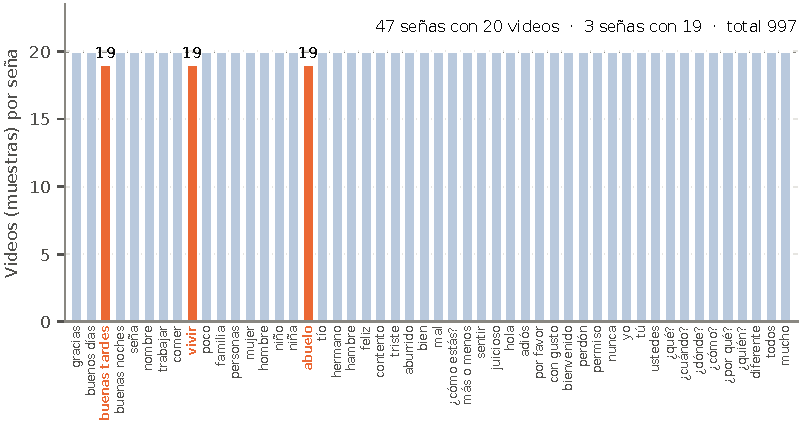
\includegraphics[width=\linewidth,height=5.3cm,keepaspectratio]{fig_muestras_por_clase.pdf}
\end{column}
\begin{column}{0.32\textwidth}
\small
\begin{itemize}\setlength\itemsep{4pt}
  \item 47 señas con 20 videos y 3 con 19: «buenas tardes», «vivir» y «abuelo».
  \item Diferencia máxima entre clases: \textbf{1 video (5 \%)}.
  \item Por persona: 200 / 199 / 198 / 200 / 200 videos (0000 a 0004).
  \item «20 por clase» son videos del corpus; la red ve además copias transformadas (pág.~\pageref{fr:receta}), iguales para todas las clases.
\end{itemize}
\end{column}
\end{columns}
\fuente{D-06; figura y conteo por persona: guiones/figuras\_datos.py sobre bitacora\_integridad.json menos las excluidas de D-06 (cuadra con data/partitions/loso\_5\_pliegues.json).}
\end{frame}

% =====================================================================
\begin{frame}{¿Qué es una muestra? Un video completo, no un cuadro}\label{fr:muestra}
\flujo{5}
\centering
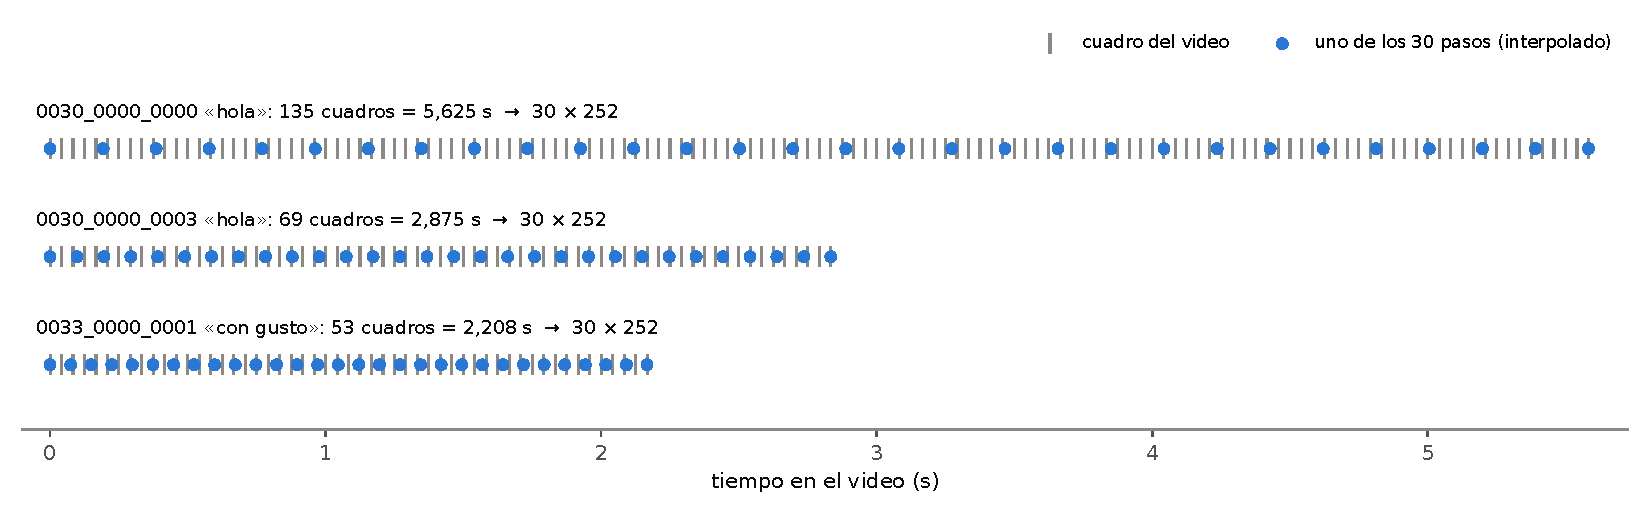
\includegraphics[width=\linewidth,height=3.35cm,keepaspectratio]{escritorio_e_duraciones.pdf}

\vspace{0.05cm}
\begin{tikzpicture}[
  c/.style={draw=azul,fill=azulclaro!55,rounded corners=2pt,align=center,font=\sffamily\scriptsize,minimum height=0.95cm,inner sep=3pt},
  fl/.style={-{Stealth[length=1.6mm]},thick,azul!80}]
  \node[c,text width=3.1cm] (a) {\textbf{1 video = 1 seña}\\ dura T cuadros\\ (40 a 135 en el corpus)};
  \node[c,text width=3.4cm,right=0.9cm of a] (b) {\textbf{Remuestreo}\\ interpolación lineal\\ a 30 pasos + velocidades};
  \node[c,text width=3.4cm,right=0.9cm of b,draw=naranja,fill=naranja!12] (d) {\textbf{1 muestra}\\ matriz 30 $\times$ 252\\ con la etiqueta de la seña};
  \draw[fl] (a) -- (b); \draw[fl] (b) -- (d);
\end{tikzpicture}

\vspace{0.1cm}
\begin{clave}[fontupper=\footnotesize]
Un video corto y uno largo producen \textbf{la misma forma} de muestra. Por eso la duración no cambia cuántas muestras tiene cada clase: 20 por seña (19 en tres).
\end{clave}
\fuente{Figura y duraciones: figuras/prueba\_escritorio.json (corridas 0-2); rango 40-135: models/canonico\_holistic\_mascara\_manos/corrida\_2026-09-15.log; src/train\_final\_100.py resample\_sequence (l. 106-114) y add\_velocity (l. 117-120); procedencia del modelo canónico (seq\_length 30, n\_rasgos\_entrada 252).}
\end{frame}

% =====================================================================
\begin{frame}{Si se contaran cuadros habría desbalance; pero el modelo cuenta videos}\label{fr:cuadros}
\flujo{5}
\begin{columns}[c]
\begin{column}{0.62\textwidth}
\centering
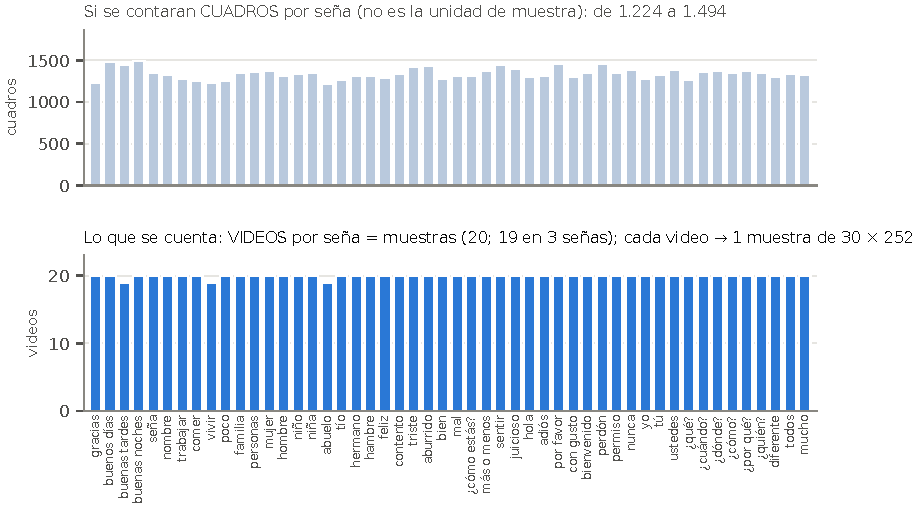
\includegraphics[width=\linewidth,height=5.6cm,keepaspectratio]{fig_cuadro_vs_video.pdf}
\end{column}
\begin{column}{0.36\textwidth}
\small
\begin{itemize}\setlength\itemsep{4pt}
  \item Arriba: si cada cuadro fuera una muestra, cada seña tendría entre \textbf{1.224} («abuelo») y \textbf{1.494} («buenas noches») cuadros; 67.145 en total (997 videos).
  \item Abajo: lo que de verdad se cuenta. Cada video se convierte en \textbf{una} matriz de 30 $\times$ 252.
  \item La red nunca recibe un cuadro suelto como ejemplo: recibe la seña entera, en 30 pasos.
\end{itemize}
\end{column}
\end{columns}
\fuente{guiones/figuras\_datos.py (fig\_cuadro\_vs\_video) sobre bitacora\_integridad.json, 997 videos; procedencia del modelo canónico.}
\end{frame}

% =====================================================================
\section{De la imagen a los números}
\begin{frame}{Qué ve la máquina en un cuadro: puntos, 21 por mano}\label{fr:puntos}
\flujo{2}
\begin{columns}[T]
\begin{column}{0.56\textwidth}
\centering
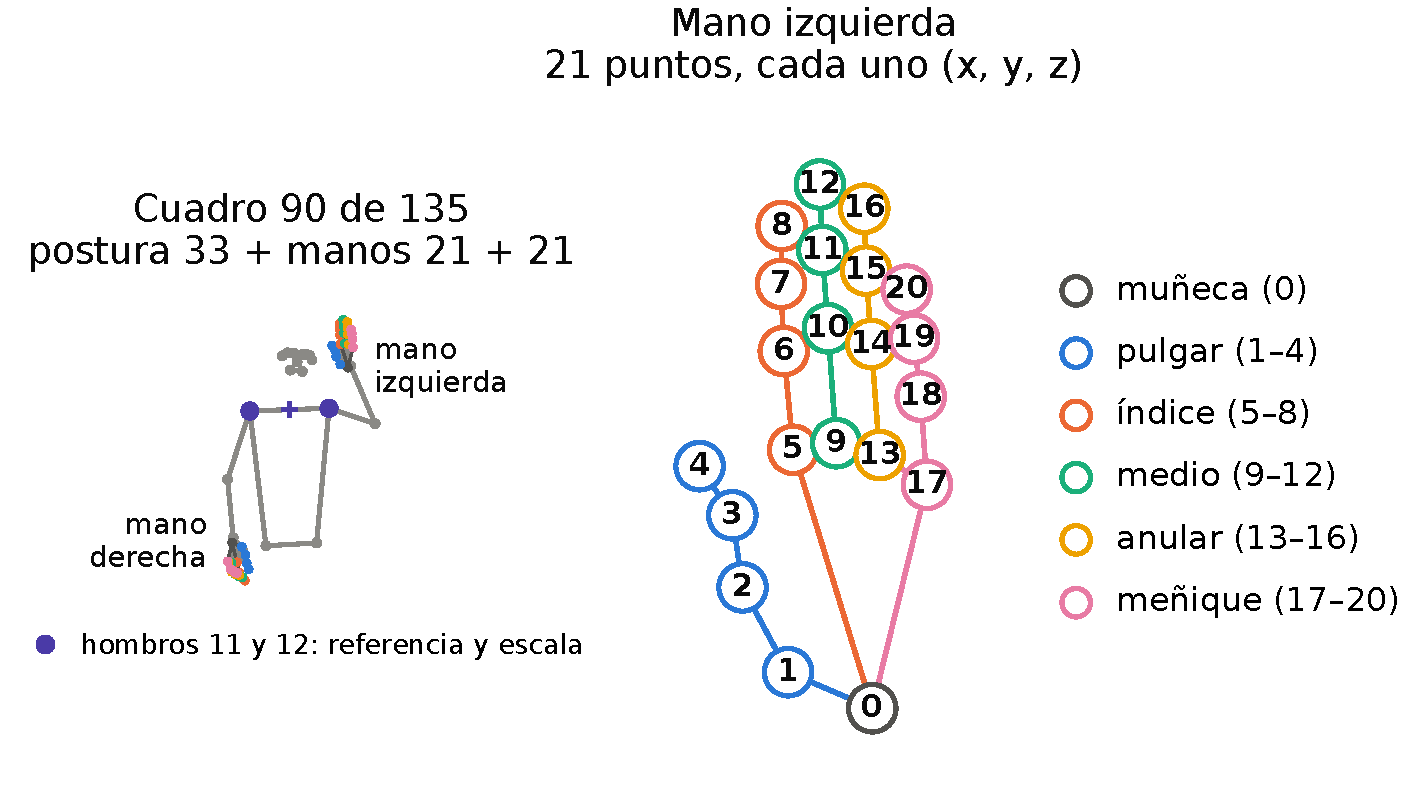
\includegraphics[width=\linewidth,height=5.0cm,keepaspectratio]{escritorio_a_esqueleto_0030_0000_0000.pdf}\\[1pt]
{\fontsize{6.5}{7.5}\selectfont\color{gris}«hola» (0030\_0000\_0000): solo el esqueleto, sin imagen de la persona. Su mano izquierda aparece a la derecha de la imagen.\par}
\end{column}
\begin{column}{0.42\textwidth}
\begin{defi}[fontupper=\scriptsize]
\textbf{Punto clave} (\emph{keypoint} o \emph{landmark}): la posición (x, y, z) de un lugar del cuerpo, p. ej. la punta del índice, que MediaPipe estima en cada cuadro.
\end{defi}
\footnotesize
\begin{itemize}\setlength\itemsep{2pt}
  \item Se procesan \textbf{todos los cuadros}: 67.328 en los 1.000 videos del depósito, 0 fallidos (24 fps; en vivo, 30,4 fps).
  \item Por cuadro, \textbf{543 puntos}: postura 33 + rostro 468 + mano izq. 21 + mano der. 21.
  \item Mano = muñeca (0) + 4 puntos por dedo = 21; x e y en fracción del ancho y alto de la imagen.
  \item Si una mano no se ve, no hay puntos de esa mano: su bloque valdrá 0 (pág.~\pageref{fr:norm}).
\end{itemize}
\end{column}
\end{columns}
\fuente{D-05 (MediaPipe 0.10.35 HolisticLandmarker); N-21 (67.328 cuadros, 0 fallidos); prueba\_escritorio.json (etapa 2, figura\_esqueleto: cuadro 90); caracterizacion.md §6; N-26 y N-52 (30,4 fps).}
\end{frame}

% =====================================================================
\begin{frame}{Normalización: dónde está la persona no debe importar}\label{fr:norm}
\flujo{3}
\begin{columns}[T]
\begin{column}{0.5\textwidth}
\centering
\begin{tikzpicture}[scale=0.95,
  persona/.pic={
    \draw[thick,black!70] (0,0.62) circle (0.17);
    \draw[thick,black!70] (-0.35,0.3) -- (-0.28,-0.45) -- (0.28,-0.45) -- (0.35,0.3);
    \draw[thick,black!70] (-0.35,0.3) -- (-0.52,-0.12) -- (-0.44,-0.5);
    \draw[very thick,naranja] (0.35,0.3) -- (0.62,0.55) -- (0.66,0.92);
    \draw[very thick,azul] (-0.35,0.3) -- (0.35,0.3);
    \fill[azul] (-0.35,0.3) circle (0.055) (0.35,0.3) circle (0.055);
    \fill[black] (0,0.3) circle (0.035);}]
  % imagen original
  \draw[gris,fill=grisclaro] (0,0) rectangle (3.4,2.6);
  \node[font=\sffamily\tiny,text=gris,anchor=north west] at (0,2.6) {imagen de la cámara};
  \pic[scale=1.25] at (0.9,1.05) {persona};
  \pic[scale=0.55] at (2.7,1.45) {persona};
  \node[font=\sffamily\tiny,align=center] at (0.9,0.18) {cerca};
  \node[font=\sffamily\tiny,align=center] at (2.7,0.9) {lejos};
  % flecha
  \draw[-{Stealth[length=2mm]},thick,azul] (3.55,1.3) -- (4.25,1.3) node[midway,above,font=\sffamily\tiny,text=azul]{normalizar};
  % normalizado
  \begin{scope}[shift={(5.5,1.1)}]
    \draw[gris!60,->] (-1.1,0) -- (1.1,0) node[right,font=\tiny]{x'};
    \draw[gris!60,->] (0,-0.9) -- (0,1.35) node[above,font=\tiny]{y'};
    \pic[scale=1.3] at (0,-0.39) {persona};
    \node[font=\sffamily\tiny,align=center,text=azul] at (0,-1.15) {ancho de hombros = 1};
  \end{scope}
\end{tikzpicture}

\vspace{0.05cm}
\small
\[
x' = \frac{x - x_{\text{centro de hombros}}}{d_{\text{hombros}}}
\]
\vspace{-0.25cm}
{\scriptsize Igual para $y$ y $z$; $d$ es la distancia entre los hombros en el plano x-y.\par}
\end{column}
\begin{column}{0.48\textwidth}
\footnotesize
\begin{itemize}\setlength\itemsep{2pt}
  \item Centro: punto medio de los hombros (puntos 11 y 12 de la postura). Escala: su distancia. Unidad: \textbf{anchos de hombro}.
  \item \textbf{Ejemplo real} («hola», cuadro 67, muñeca derecha):\\
  $x' = (0{,}4523 - 0{,}5247)/0{,}1139 = -0{,}6356$\\
  $y' = (0{,}8852 - 0{,}5705)/0{,}1139 = 2{,}7628$\\
  (la muñeca cuelga 2,76 anchos de hombro por debajo del centro).
  \item \textbf{Mano no vista} (regla «máscara»): su bloque vale 0 después de normalizar. En «hola» pasa en 1 cuadro.
  \item Lo mismo en el corpus y en el prototipo en vivo.
\end{itemize}
\begin{clave}[fontupper=\scriptsize]
Por construcción, mover o alejar a la persona no cambia $x'$ ni $y'$. Cuánto compensa esto en vivo no se ha medido.
\end{clave}
\end{column}
\end{columns}
\fuente{procedencia del modelo canónico (shoulder\_centered\_scaled); src/preprocess\_lsc50.py l. 496-500; N-11; D-07; ejemplo: prueba\_escritorio.json → corridas[0].normalizacion.ejemplo.}
\end{frame}

% =====================================================================
\begin{frame}{Temporalidad (1): las señas no duran lo mismo}\label{fr:tempo1}
\flujo{5}
\begin{columns}[c]
\begin{column}{0.6\textwidth}
\centering
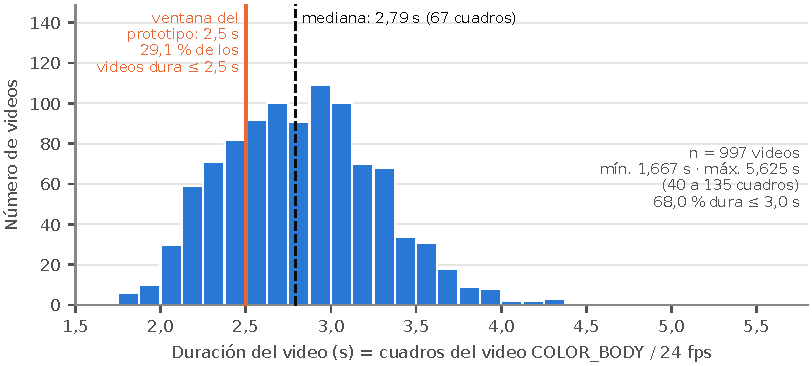
\includegraphics[width=\linewidth,height=4.9cm,keepaspectratio]{fig_duracion_clips.pdf}
\end{column}
\begin{column}{0.38\textwidth}
\small
\begin{itemize}\setlength\itemsep{3pt}
  \item 997 videos: de \textbf{1,667 s} (40 cuadros) a \textbf{5,625 s} (135); mediana \textbf{2,79 s} (67 cuadros).
  \item Cuadros = duración $\times$ 24 fps.
  \item Cada persona tiene su ritmo: mediana 2,96 / 2,92 / 2,75 / 2,33 / 3,00 s (personas 0000 a 0004).
  \item Una seña se reconoce por el movimiento, no por un cuadro: la red necesita la secuencia completa.
  \item En vivo la ventana dura 2,5 s: el 29,1 \% de los videos cabe en 2,5 s y el 68,0 \% en 3,0 s.
\end{itemize}
\end{column}
\end{columns}
\fuente{guiones/figuras\_datos.py sobre bitacora\_integridad.json (video COLOR\_BODY, 997 videos); caracterizacion.md §5; N-48 (con 1.000 videos: 29,2 \% y 68,0 \%); src/realtime.py (ventana 2,5 s).}
\end{frame}

% =====================================================================
\begin{frame}{Temporalidad (2): cualquier duración se reparte en 30 pasos}\label{fr:tempo2}
\flujo{5}
\begin{columns}[T]
\begin{column}{0.56\textwidth}
\centering
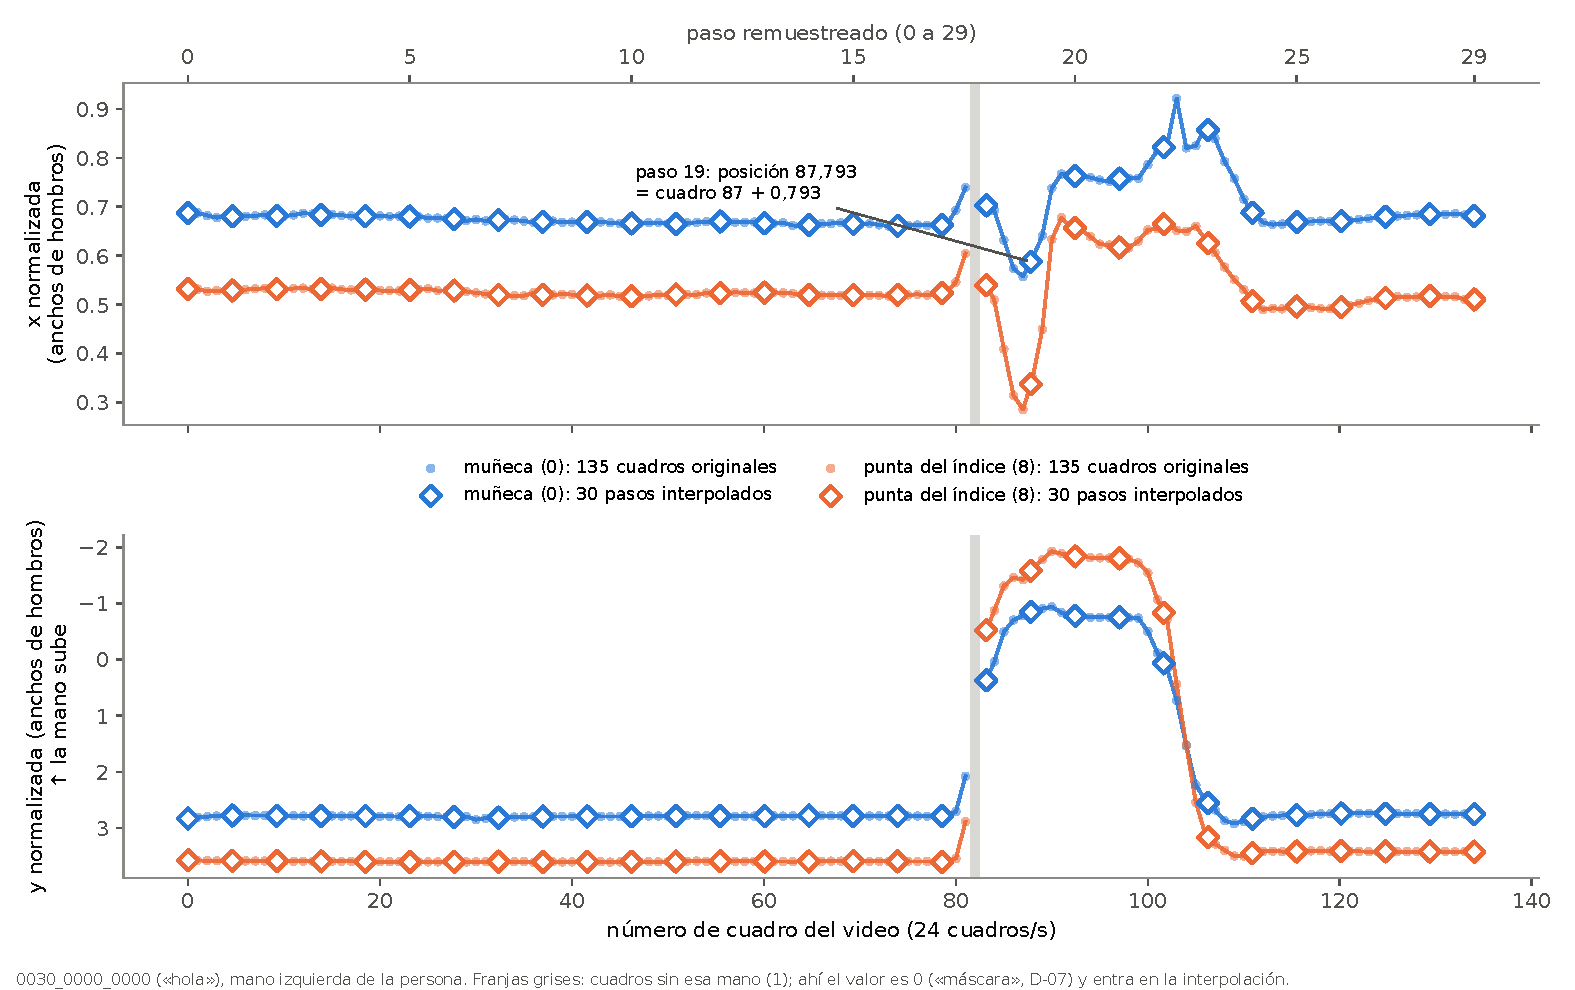
\includegraphics[width=\linewidth,height=5.3cm,keepaspectratio]{escritorio_b_interpolacion_0030_0000_0000.pdf}
\end{column}
\begin{column}{0.42\textwidth}
\footnotesize
\textbf{\color{azul}Regla}: el paso $j$ (0 a 29) cae en la posición
\[ \text{pos}_j = j\cdot\frac{T-1}{29} \]
Si cae entre dos cuadros, se toma el punto intermedio en línea recta entre ellos.\par\smallskip
\textbf{\color{azul}Cuenta completa} («hola», T = 135 cuadros; x de la muñeca izquierda):
\begin{itemize}\setlength\itemsep{1pt}
  \item paso 19: $19\cdot 134/29 = 87{,}79310$ $\rightarrow$ entre el cuadro 87 y el 88, fracción 0,79310.
  \item $x = 0{,}55756 + 0{,}79310\cdot(0{,}59547 - 0{,}55756) = 0{,}58763$.
  \item El código (\texttt{resample\_sequence}) da 0,58763.
\end{itemize}
\begin{clave}[fontupper=\scriptsize]
Los rombos (30 pasos) caen sobre la misma curva que los 135 cuadros: se conserva la \textbf{forma} del movimiento y se descarta la duración.
\end{clave}
\end{column}
\end{columns}
\fuente{src/train\_final\_100.py:106-114 (np.linspace + np.interp); prueba\_escritorio.json → corridas[0].ejemplo; figura: guiones/prueba\_escritorio.py.}
\end{frame}

% =====================================================================
\begin{frame}{Las 252 características: 126 de posición + 126 de velocidad}\label{fr:252}
\flujo{6}
{\footnotesize\raggedright De los 543 puntos de MediaPipe se guardan \textbf{135} (postura 33 + manos 42 + cejas y labios 60) $\times$ 3 coordenadas = \textbf{405 números por cuadro}; los otros 408 puntos del rostro no se guardan.\par}
\vspace{0.1cm}
\centering
\begin{tikzpicture}[x=0.03cm,
  seg/.style={draw=white,line width=0.6pt,minimum height=0.5cm,inner sep=0,font=\sffamily\fontsize{6.5}{7.5}\selectfont,align=center},
  lab/.style={font=\sffamily\scriptsize,anchor=east,align=right,text width=2.1cm}]
  % Fila 1: 405 por cuadro
  \node[lab] at (-5,0) {\textbf{Fila por cuadro}\\405 números};
  \node[seg,fill=gris!30,minimum width=99*0.03cm,anchor=west] at (0,0) {postura 99};
  \node[seg,fill=azul,text=white,minimum width=63*0.03cm,anchor=west] at (99,0) {mano izq. 63};
  \node[seg,fill=azul!70,text=white,minimum width=63*0.03cm,anchor=west] at (162,0) {mano der. 63};
  \node[seg,fill=gris!30,minimum width=180*0.03cm,anchor=west] at (225,0) {cejas y labios 180 (no entran, D-08)};
  % Fila 2: 126
  \node[lab] at (-5,-1.1) {\textbf{Posición}\\126 = 2 $\times$ 21 $\times$ 3};
  \node[seg,fill=azul,text=white,minimum width=63*0.03cm,anchor=west] (pi) at (0,-1.1) {mano izq. 63};
  \node[seg,fill=azul!70,text=white,minimum width=63*0.03cm,anchor=west] (pd) at (63,-1.1) {mano der. 63};
  \draw[-{Stealth[length=1.5mm]},gris] (130,-0.28) -- (63,-0.8);
  \node[font=\sffamily\fontsize{6.5}{7.5}\selectfont,anchor=west,align=left] at (132,-1.1)
     {63 = 21 puntos $\times$ (x, y, z): \texttt{p0x p0y p0z p1x \dots\ p20z}};
  % Fila 3: 252
  \node[lab] at (-5,-2.2) {\textbf{Un paso}\\252 números};
  \node[seg,fill=azul,text=white,minimum width=63*0.03cm,anchor=west] at (0,-2.2) {pos. izq. 63};
  \node[seg,fill=azul!70,text=white,minimum width=63*0.03cm,anchor=west] at (63,-2.2) {pos. der. 63};
  \node[seg,fill=naranja,text=white,minimum width=63*0.03cm,anchor=west] at (126,-2.2) {vel. izq. 63};
  \node[seg,fill=naranja!70,text=white,minimum width=63*0.03cm,anchor=west] at (189,-2.2) {vel. der. 63};
  \node[font=\sffamily\fontsize{6.5}{7.5}\selectfont,anchor=west,align=left] at (258,-2.2)
     {velocidad $v_j = p_j - p_{j-1}$ (en el paso 0, $v_0 = 0$)};
  % Fila 4: matriz
  \node[lab] at (-5,-3.35) {\textbf{Un video}\\30 pasos};
  \foreach \k in {0,...,5} \draw[fill=azulclaro,draw=azul!60] (\k*2.2,-3.1-\k*0.07) rectangle ++(252*0.33,-0.28);
  \node[font=\sffamily\fontsize{6.5}{7.5}\selectfont,anchor=west,align=left] at (100,-3.4)
     {$\times$ 30 pasos $\rightarrow$ \textbf{matriz 30 $\times$ 252 = 7.560 números}: la entrada de la red para una seña};
\end{tikzpicture}

\vspace{0.2cm}
\footnotesize
\begin{columns}[T]
\begin{column}{0.49\textwidth}
\begin{itemize}\setlength\itemsep{1pt}
  \item \textbf{Posición}: dónde está cada punto de cada mano, en anchos de hombro.
  \item \textbf{Velocidad}: cuánto se movió esa misma coordenada desde el paso anterior.
\end{itemize}
\end{column}
\begin{column}{0.49\textwidth}
\begin{itemize}\setlength\itemsep{1pt}
  \item Ejemplo real («hola», paso 19, x de la muñeca izq.): $v_{19} = 0{,}58763 - 0{,}70290 = -0{,}11527$.
  \item La entrada así construida es idéntica (diferencia 0) a la que usó el entrenamiento.
\end{itemize}
\end{column}
\end{columns}
\fuente{src/representacion.py (columnas 99:225, «manos»; «cejas\_labios» = 20 de cejas + 40 de labios); src/train\_final\_100.py:117-120 (add\_velocity); procedencia del modelo canónico (n\_rasgos\_por\_paso 126, n\_rasgos\_entrada 252); prueba\_escritorio.json → corridas[0].ejemplo y entrenador.dif\_max; D-08, N-30.}
\end{frame}

% =====================================================================
\begin{frame}{Así se ve la entrada real de «hola»: 30 pasos $\times$ 252 números}\label{fr:matriz}
\flujo{6}
\centering
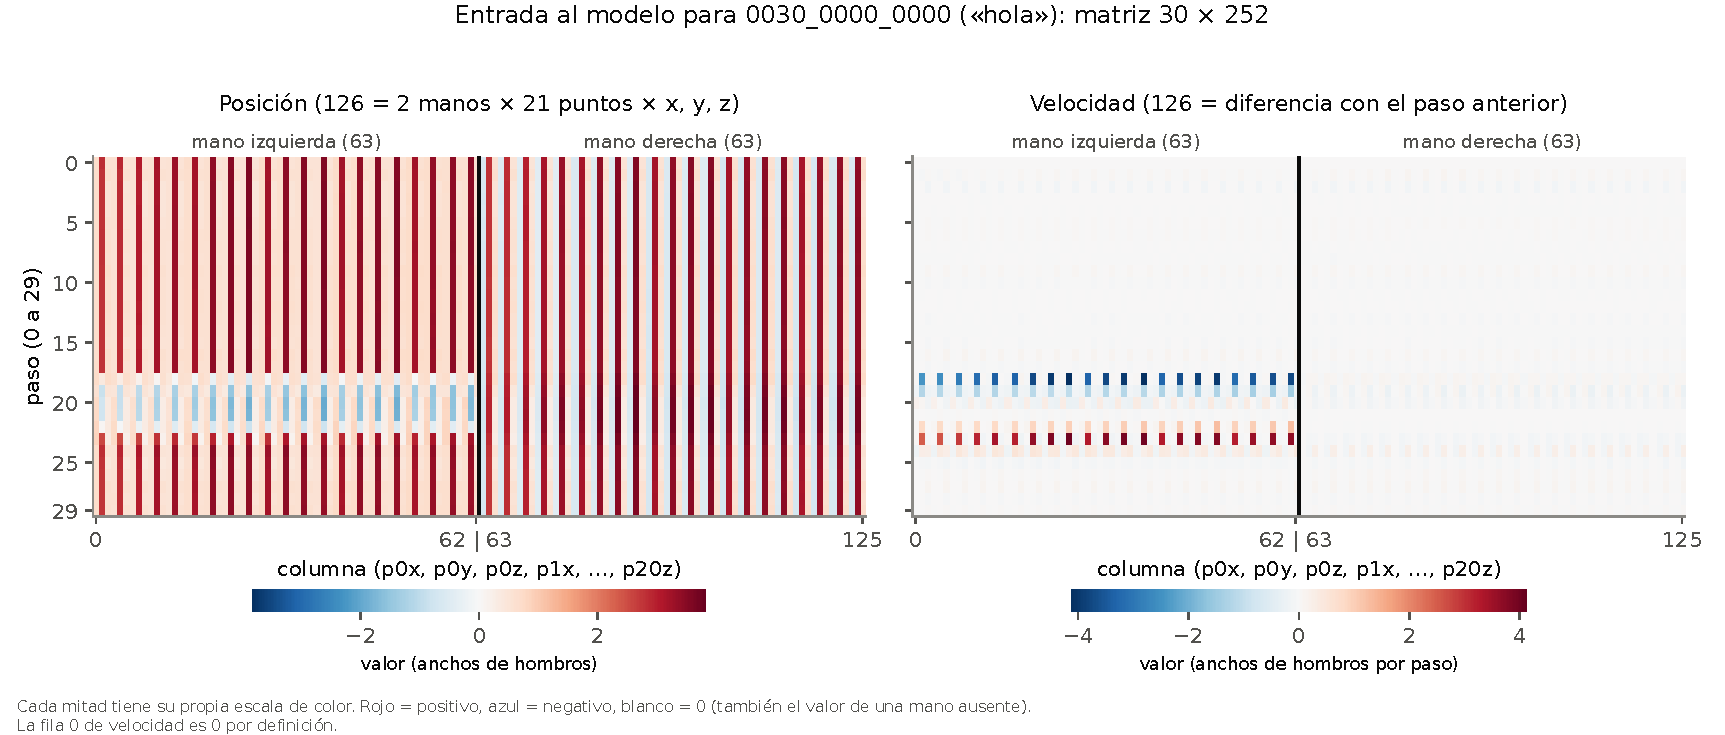
\includegraphics[width=\linewidth,height=4.6cm,keepaspectratio]{escritorio_c_matriz_entrada_0030_0000_0000.pdf}

\vspace{0.05cm}
\begin{columns}[T]
\begin{column}{0.49\textwidth}
\footnotesize
\begin{itemize}\setlength\itemsep{1pt}
  \item Filas: los 30 pasos. Columnas: posición (izquierda) y velocidad (derecha).
  \item La velocidad solo se «enciende» en los pasos $\approx$18 a 23, cuando la mano izquierda sube y baja.
\end{itemize}
\end{column}
\begin{column}{0.49\textwidth}
\footnotesize
\begin{itemize}\setlength\itemsep{1pt}
  \item Este video es el más largo del corpus (135 cuadros): la mano está arriba solo en los cuadros 83 a 104; el resto es reposo.
  \item Cada mitad tiene su propia escala de color; el blanco (0) es también el valor de una mano ausente.
\end{itemize}
\end{column}
\end{columns}
\fuente{figuras/escritorio\_c\_matriz\_entrada\_0030\_0000\_0000.pdf (guiones/prueba\_escritorio.py); tramo 83-104: cálculo propio sobre data/processed\_holistic\_mascara\_rostro/samples/0030\_0000\_0000.npy (criterio: y de la muñeca izquierda $<$ 2 anchos de hombro).}
\end{frame}

% =====================================================================
\section{El modelo}
\begin{frame}{Sí es una LSTM: Conv1D + LSTM bidireccional + atención, en TensorFlow/Keras}\label{fr:red}
\flujo{7}
\centering
\begin{tikzpicture}[
  b/.style={draw=morado,fill=morado!10,rounded corners=2pt,align=center,font=\sffamily\small,
            text width=2.4cm,minimum height=1.25cm,inner sep=3pt,
            execute at begin node={\hyphenpenalty=10000\exhyphenpenalty=10000}},
  io/.style={b,draw=azul,fill=azulclaro!60},
  bsal/.style={b,draw=naranja,fill=naranja!15},
  fsh/.style={font=\ttfamily\small\bfseries,text=naranja!85!black},
  fl/.style={-{Stealth[length=2mm]},thick,morado!80},
  nota/.style={font=\sffamily\scriptsize,text=gris,align=center,text width=3cm}]
  % fila 1: lectura de la secuencia
  \node[io] (in) at (0,0) {\textbf{Entrada}\\ un video};
  \node[b,right=0.65cm of in] (cv) {\textbf{2 capas Conv1D}\\ ventanas de 3 pasos};
  \node[b,right=0.65cm of cv] (l1) {\textbf{LSTM}\\ \textbf{bidireccional 1}};
  \node[b,right=0.65cm of l1] (l2) {\textbf{LSTM}\\ \textbf{bidireccional 2}};
  \foreach \n/\t in {in/30 $\times$ 252,cv/30 $\times$ 128,l1/30 $\times$ 256,l2/30 $\times$ 128}
    \node[fsh,below=1pt of \n] (f\n) {\t};
  \draw[fl] (in) -- (cv); \draw[fl] (cv) -- (l1); \draw[fl] (l1) -- (l2);
  \node[nota,above=2pt of cv] {patrones cortos de movimiento};
  \node[nota,above=2pt of l1,xshift=1.45cm,text width=5.5cm] {recorren los 30 pasos hacia adelante y hacia atrás: \textbf{aquí está la temporalidad}};
  % fila 2: resumen y decisión
  \node[b,text width=2.1cm,minimum height=0.5cm,below=0.75cm of fl2,xshift=-0.2cm] (at) {atención};
  \node[b,text width=2.1cm,minimum height=0.5cm,below=0.1cm of at] (pr) {promedio};
  \node[b,text width=2.1cm,minimum height=0.5cm,below=0.1cm of pr] (mx) {máximo};
  \node[draw=morado!60,dashed,rounded corners=2pt,fit=(at)(mx),inner sep=3pt] (grp) {};
  \node[fsh,right=2pt of grp,align=left] (fr) {3 $\times$ 128};
  \node[b,left=1.0cm of pr] (cc) {\textbf{Resumen}\\ del video};
  \node[b,left=0.65cm of cc] (d1) {\textbf{2 capas densas}\\ 256 y 128};
  \node[bsal,left=0.65cm of d1] (sm) {\textbf{Softmax}\\ 50 señas};
  \node[fsh,below=1pt of cc] {384};
  \node[fsh,below=1pt of d1] {256 $\rightarrow$ 128};
  \node[fsh,below=1pt of sm] {50 probabilidades};
  \draw[fl] (fl2.south) -- (fl2.south |- grp.north);
  \draw[fl] (at.west) -- (cc.east |- at.west);
  \draw[fl] (pr.west) -- (cc.east);
  \draw[fl] (mx.west) -- (cc.east |- mx.west);
  \draw[fl] (cc) -- (d1); \draw[fl] (d1) -- (sm);
  \node[nota,above=2pt of cc,text width=3.2cm] {¿qué momentos importan?};
  \node[nota,above=2pt of sm,text width=3.2cm] {la mayor es la seña};
\end{tikzpicture}

\vspace{0.05cm}
{\small TensorFlow 2.21 / Keras 3.13 $\cdot$ \textbf{713.011 pesos entrenables} $\cdot$ parámetros por capa en A1 (pág.~\pageref{fr:capas})\par}
\fuente{modelo\_canonico.keras cargado y comparado capa por capa con build\_model(30, 252, 50) de src/train\_final\_100.py (l. 149-185): figuras/tabla\_capas\_modelo.json; versiones: models/canonico\_holistic\_mascara\_manos/resultados.json → entorno; N-31. Diagrama con parámetros por bloque: figuras/arquitectura\_modelo.pdf (guiones/diagrama\_arquitectura.py).}
\end{frame}

% =====================================================================
\begin{frame}{Qué hace cada bloque de la red, y qué se entrena y qué no}\label{fr:bloques}
\flujo{7}
\begin{columns}[T]
\begin{column}{0.6\textwidth}
\footnotesize
\renewcommand{\arraystretch}{1.25}
\hyphenpenalty=10000
\begin{tabularx}{\linewidth}{@{}>{\leavevmode\color{azul}\bfseries\raggedright}p{2.05cm} >{\raggedright\arraybackslash\leavevmode}X@{}}
Conv1D (k = 3) & Mira ventanas de 3 pasos seguidos y detecta patrones cortos de movimiento; 128 detectores. \\
LSTM bidireccional & Recorre los 30 pasos hacia adelante y hacia atrás con memoria: el valor de un paso depende de lo que vino antes y después. \textbf{Aquí se maneja la temporalidad.} \\
Atención & Da a cada paso un peso (suman 1) y promedia; junto al promedio simple y al máximo forma un resumen de 384 números del video. \\
Densas + softmax & Convierten el resumen en 50 probabilidades que suman 1 (eso hace la capa softmax); la mayor es la seña. \\
\color{gris}BatchNorm, Dropout & \color{gris}Estabilizan el entrenamiento; Dropout apaga neuronas al azar al entrenar para que no memorice. \\
\end{tabularx}
\end{column}
\begin{column}{0.38\textwidth}
\centering
\begin{tikzpicture}[
  c/.style={rounded corners=2pt,align=center,font=\sffamily\scriptsize,text width=4.3cm,inner sep=4pt,
           execute at begin node={\hyphenpenalty=10000\exhyphenpenalty=10000}}]
  \node[c,draw=gris,fill=grisclaro] (mp) {\textbf{MediaPipe Holistic 0.10.35}\\ preentrenado por Google\\ \textbf{fijo: no se entrena}};
  \node[c,draw=morado,fill=morado!12,below=0.55cm of mp] (red) {\textbf{Red Conv1D + BiLSTM + atención}\\ \textbf{713.011 pesos} que se ajustan con los videos de LSC50\\ (+ 1.280 valores no entrenables)};
  \draw[-{Stealth[length=1.6mm]},thick,azul] (mp) -- node[right,font=\sffamily\tiny]{puntos} (red);
\end{tikzpicture}

\vspace{0.15cm}
\scriptsize
{\raggedright\hyphenpenalty=10000 \textbf{Cómo aprende}: compara sus 50 probabilidades con la seña real (entropía cruzada) y corrige los pesos con el optimizador Adam, lote a lote (64 secuencias). Todo en CPU.\par}
\end{column}
\end{columns}
\fuente{src/train\_final\_100.py build\_model y entrenar\_semilla (l. 436-451); figuras/tabla\_capas\_modelo.json (totales); D-05; anteproyecto 06\_alcances.tex:27-28 (CPU).}
\end{frame}

% =====================================================================
\begin{frame}{Entrenamiento, validación y prueba: la prueba no decide nada}\label{fr:particion}
\flujo{7}
\centering
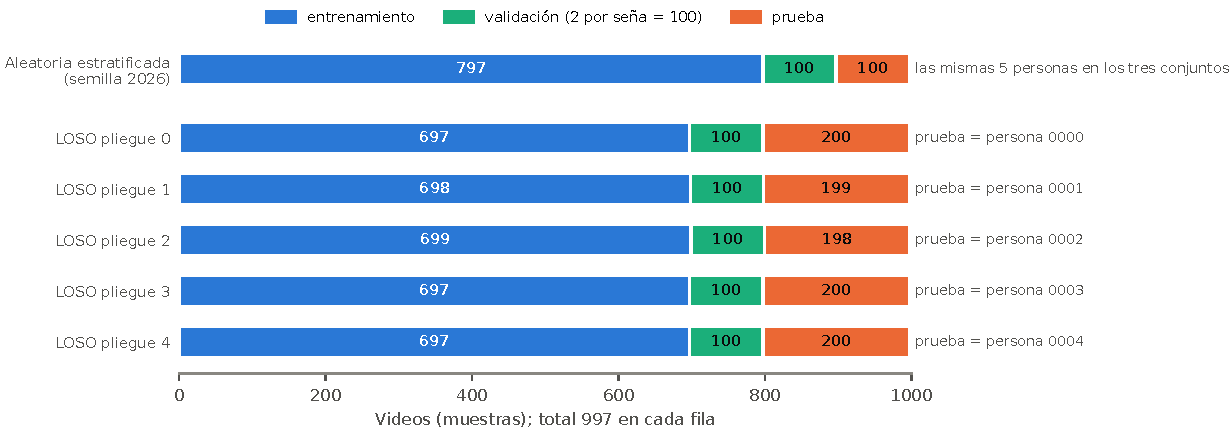
\includegraphics[width=\linewidth,height=3.45cm,keepaspectratio]{fig_particiones.pdf}

\vspace{0.05cm}
\begin{columns}[T]
\begin{column}{0.325\textwidth}
\begin{defi}[fontupper=\scriptsize]
\textbf{Entrenamiento}: los videos con los que la red ajusta sus pesos (797 en el esquema aleatorio).
\end{defi}
\end{column}
\begin{column}{0.325\textwidth}
\begin{defi}[fontupper=\scriptsize]
\textbf{Validación}: videos apartados que solo deciden cuándo parar y qué pesos se guardan (100; 2 por seña).
\end{defi}
\end{column}
\begin{column}{0.325\textwidth}
\begin{defi}[fontupper=\scriptsize]
\textbf{Prueba}: videos que se evalúan una sola vez, al final (100; 2 por seña).
\end{defi}
\end{column}
\end{columns}
\vspace{0.05cm}
{\raggedright\scriptsize
Partición aleatoria estratificada con semilla 2026, fijada antes de entrenar: 16/2/2 por seña (15/2/2 en las tres de 19). LOSO = dejar una persona fuera (pág.~\pageref{fr:esquemas}): en el pliegue $k$ la prueba son todos los videos de la persona 000$k$. Ningún duplicado entra en ningún conjunto.\par}
\fuente{data/partitions/aleatoria\_80\_10\_10.json y loso\_5\_pliegues.json (conteos, criterio, uso\_del\_test); D-06; figura: guiones/figuras\_datos.py.}
\end{frame}

% =====================================================================
\begin{frame}{Receta del entrenamiento: 797 videos se vuelven 7.970 secuencias}\label{fr:receta}
\flujo{7}
\begin{columns}[T]
\begin{column}{0.5\textwidth}
\small
\textbf{\color{azul}Cuatro ajustes clave}\par\smallskip
\renewcommand{\arraystretch}{1.25}
\begin{tabular}{@{}>{\bfseries}l >{\raggedright\arraybackslash}p{4.4cm}@{}}
\toprule
Optimizador & Adam, tasa inicial 0,001 \\
Lote & 64 secuencias (125 lotes por época) \\
Parada temprana & si la validación no mejora en 25 épocas; se guardan los mejores pesos \\
Aumentación & $\times$10 (a la derecha) \\
\bottomrule
\end{tabular}\par\medskip
\footnotesize 5 semillas (2026 a 2030); queda la de mejor validación: 2026 (0,96), 140 s de entrenamiento en CPU. Todos los ajustes, en A2 (pág.~\pageref{fr:hiper}).
\end{column}
\begin{column}{0.47\textwidth}
\begin{defi}[fontupper=\scriptsize]
\textbf{Época}: una pasada completa de la red por todas las secuencias de entrenamiento. \textbf{Semilla}: número que fija el azar del entrenamiento (pesos iniciales, orden de los lotes).
\end{defi}
\small
\textbf{\color{azul}Aumentación $\times$10}: cada video de entrenamiento + 9 copias con cambios pequeños (espejo, ruido, re-muestreo temporal, escala), para que la red no memorice a la persona.\par\smallskip
\footnotesize Validación y prueba \textbf{nunca} se aumentan.
\end{column}
\end{columns}
\fuente{models/canonico\_holistic\_mascara\_manos/resultados.json (configuracion, semillas, seleccion); src/train\_final\_100.py (l. 207-241 aumentación; l. 436-451 optimizador, parada y checkpoint); corrida\_2026-09-15.log; N-31. Detalle en el apéndice (pág.~\pageref{fr:hiper}).}
\end{frame}

% =====================================================================
\begin{frame}{Cómo aprendió la red: del azar a 0,96 en validación; se guardó la época 17}\label{fr:curvas}
\flujo{7}
\centering
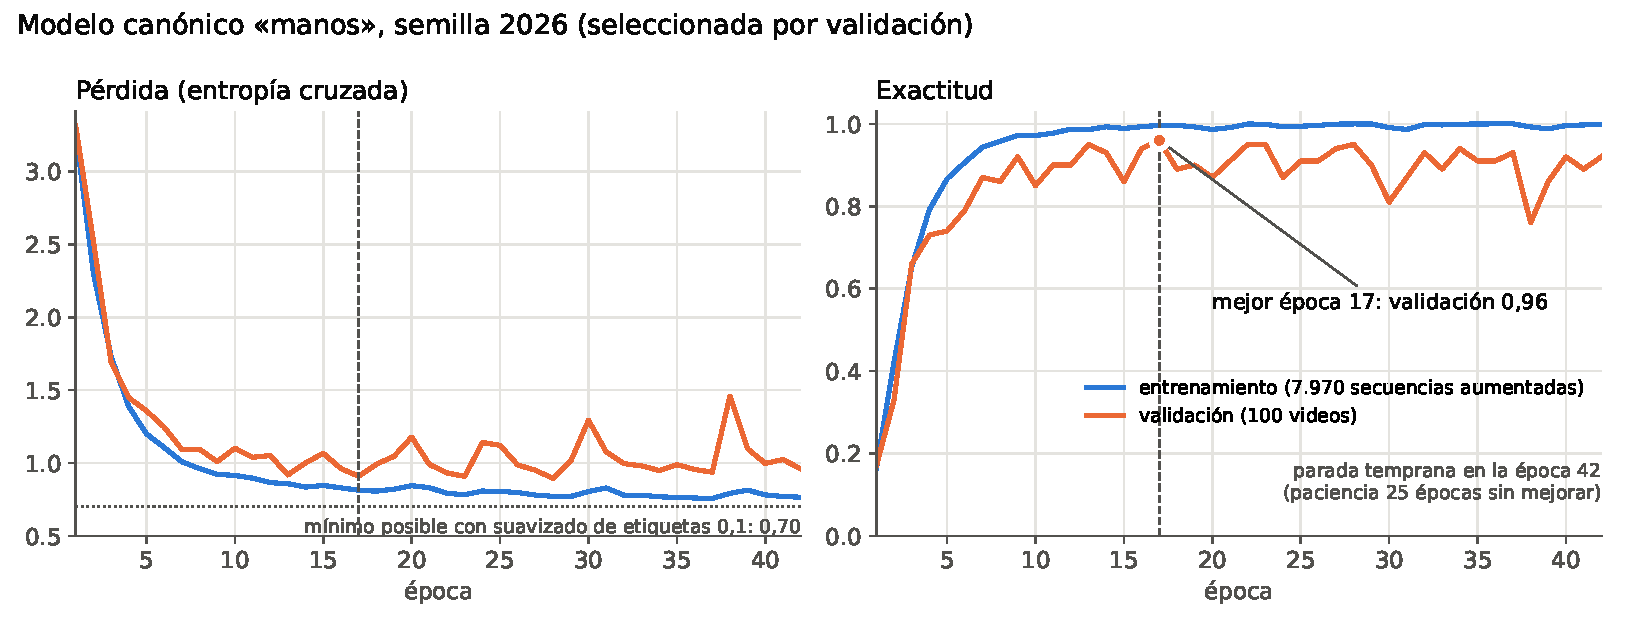
\includegraphics[width=\linewidth,height=4.1cm,keepaspectratio]{curvas_aprendizaje_semilla2026.pdf}

\vspace{0.05cm}
\begin{columns}[T]
\begin{column}{0.49\textwidth}
\footnotesize
\begin{itemize}\setlength\itemsep{1pt}
  \item Época 1: 0,17 en validación (el azar con 50 señas es 0,02).
  \item Época 17: entrenamiento 0,996, validación \textbf{0,96} $\rightarrow$ se guardan esos pesos.
  \item Se paró en la época 42: 25 épocas sin mejorar.
\end{itemize}
\end{column}
\begin{column}{0.49\textwidth}
\footnotesize
\begin{itemize}\setlength\itemsep{1pt}
  \item La validación oscila porque son 100 videos: 1 video = 1 punto porcentual.
  \item La pérdida no baja de 0,70 por el suavizado de etiquetas.
  \item Exactitud de entrenamiento: sobre secuencias aumentadas y con Dropout activo.
\end{itemize}
\end{column}
\end{columns}
\fuente{models/canonico\_holistic\_mascara\_manos/semilla\_2026/historial.json (resumen en figuras/curvas\_aprendizaje\_semilla2026.json); guion guiones/curvas\_aprendizaje.py; N-31.}
\end{frame}

% =====================================================================
\section{Prueba de escritorio}
\begin{frame}{Prueba de escritorio: el video «hola» de principio a fin}\label{fr:escritorio}
\scriptsize
\renewcommand{\arraystretch}{1.13}
\begin{tabularx}{\textwidth}{@{}c l l >{\raggedright\arraybackslash\leavevmode}X@{}}
\toprule
& \textbf{Etapa} & \textbf{Sale (forma)} & \textbf{Qué pasó con 0030\_0000\_0000 («hola», persona 0000)} \\
\midrule
1 & Video .avi & 135 cuadros 1920$\times$1080 & 24 fps $\rightarrow$ 5,625 s (el video más largo del corpus) \\
2 & MediaPipe HolisticLandmarker & 543 puntos (x, y, z) por cuadro & postura 135/135; mano izq. 134/135; mano der. 135/135 \\
3 & Fila por cuadro & \texttt{(135, 405)} & 135 de los 543 puntos $\times$ 3: postura 99 + manos 126 + cejas y labios 180 \\
4 & Normalización + «máscara» & \texttt{(135, 405)} & centrado y escala por hombros; 1 cuadro sin mano izquierda $\rightarrow$ 0 \\
5 & Solo manos & \texttt{(135, 126)} & columnas 99 a 224 \\
6 & Remuestreo & \texttt{(30, 126)} & paso $j$ en la posición $j\cdot 134/29$ \\
7 & + velocidades & \texttt{(1, 30, 252)} & idéntica a la del entrenamiento para esta muestra (diferencia 0) \\
8 & Red neuronal & 50 probabilidades & top-1 «hola» \textbf{0,902}; «¿por qué?» 0,009; «niño» 0,005 \\
9 & Umbral 0,20 + GrammarMapper & texto $\rightarrow$ voz & 0,902 $\geq$ 0,20 $\rightarrow$ aceptada $\rightarrow$ «Hola» \\
\bottomrule
\end{tabularx}

\vspace{0.15cm}
\begin{clave}[fontupper=\scriptsize]
Esta muestra se usó para entrenar el modelo: prueba que el camino funciona, no que el modelo acierte. La exactitud con personas nuevas la da el LOSO (pág.~\pageref{fr:nuevas}).
\end{clave}
\fuente{figuras/prueba\_escritorio.json (corridas[0]: video, extraccion.detecciones, formas, entrenador.dif\_max, top3, decision, enunciado); guion guiones/prueba\_escritorio.py; D-05, D-07, D-08, D-09; data/partitions/aleatoria\_80\_10\_10.json.}
\end{frame}

% =====================================================================
\begin{frame}{La salida: 50 probabilidades, y la decisión con el umbral}\label{fr:salida}
\flujo{8}
\centering
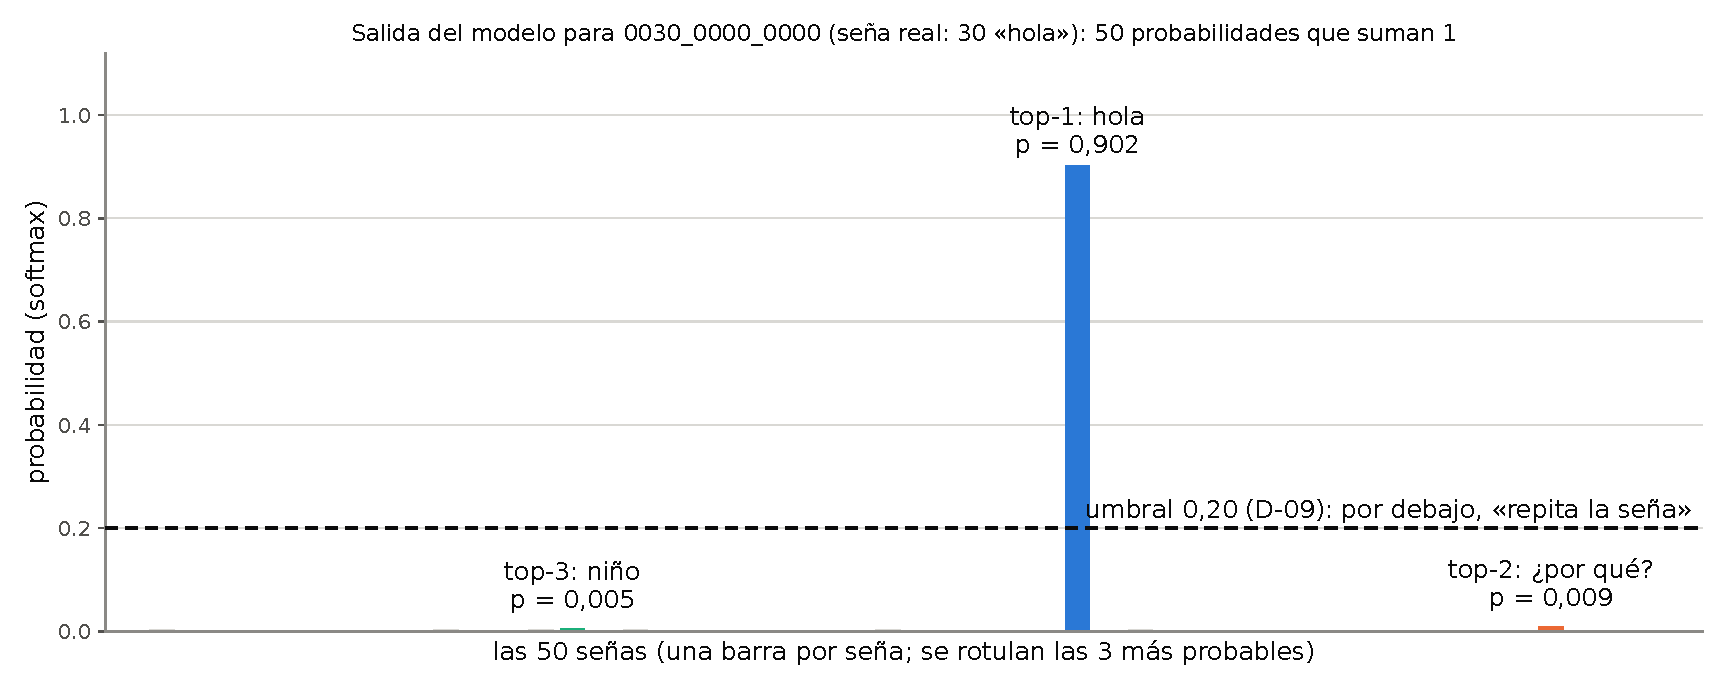
\includegraphics[width=\linewidth,height=3.85cm,keepaspectratio]{escritorio_d_probabilidades_0030_0000_0000.pdf}

\vspace{0.05cm}
\scriptsize
\renewcommand{\arraystretch}{1.08}
\begin{tabular}{@{}l l r r l l l@{}}
\toprule
Muestra & Seña & Cuadros & Segundos & Forma final & 1.ª opción (2.ª opción) & Conjunto \\
\midrule
0030\_0000\_0000 & hola & 135 & 5,625 & 30 $\times$ 252 & hola 0,902 (¿por qué? 0,009) & entrenamiento \\
0030\_0000\_0003 & hola & 69 & 2,875 & 30 $\times$ 252 & hola 0,876 (¿por qué? 0,013) & prueba \\
0033\_0000\_0001 & con gusto & 53 & 2,208 & 30 $\times$ 252 & con gusto 0,370 (sentir 0,330) & validación \\
\bottomrule
\end{tabular}

\vspace{0.1cm}
\footnotesize
Tres aciertos no son una métrica: el tercero gana a «sentir» por poco (0,370 frente a 0,330), y con 0,55 se habría pedido repetir (camino del corpus).
\fuente{figuras/prueba\_escritorio.json (corridas[0-2]: T, top3, decision); data/partitions/aleatoria\_80\_10\_10.json; D-09 (umbral 0,20); N-47 (0,55, no adoptado).}
\end{frame}

% =====================================================================
\begin{frame}{La red por dentro, con un video de prueba: «gracias» sale con 0,968}\label{fr:pasada}
\flujo{7}
\centering
\begin{tikzpicture}[
  c/.style={draw=morado,fill=morado!10,rounded corners=1.5pt,font=\ttfamily\fontsize{6.5}{7.5}\selectfont,inner sep=2.5pt,align=center},
  fl/.style={-{Stealth[length=1.3mm]},morado!80}]
  \node[c] (a) {50 cuadros\\$\times$ 126};
  \node[c,right=0.3cm of a] (b) {30 $\times$ 126};
  \node[c,right=0.3cm of b] (c) {30 $\times$ 252};
  \node[c,right=0.3cm of c] (d) {Conv1D\\30 $\times$ 128};
  \node[c,right=0.3cm of d] (e) {BiLSTM\\30 $\times$ 256};
  \node[c,right=0.3cm of e] (f) {BiLSTM\\30 $\times$ 128};
  \node[c,right=0.3cm of f] (g) {resumen\\384};
  \node[c,right=0.3cm of g,fill=naranja!15,draw=naranja] (h) {50\\probabilidades};
  \foreach \x/\y in {a/b,b/c,c/d,d/e,e/f,f/g,g/h} \draw[fl] (\x) -- (\y);
\end{tikzpicture}

\vspace{0.1cm}
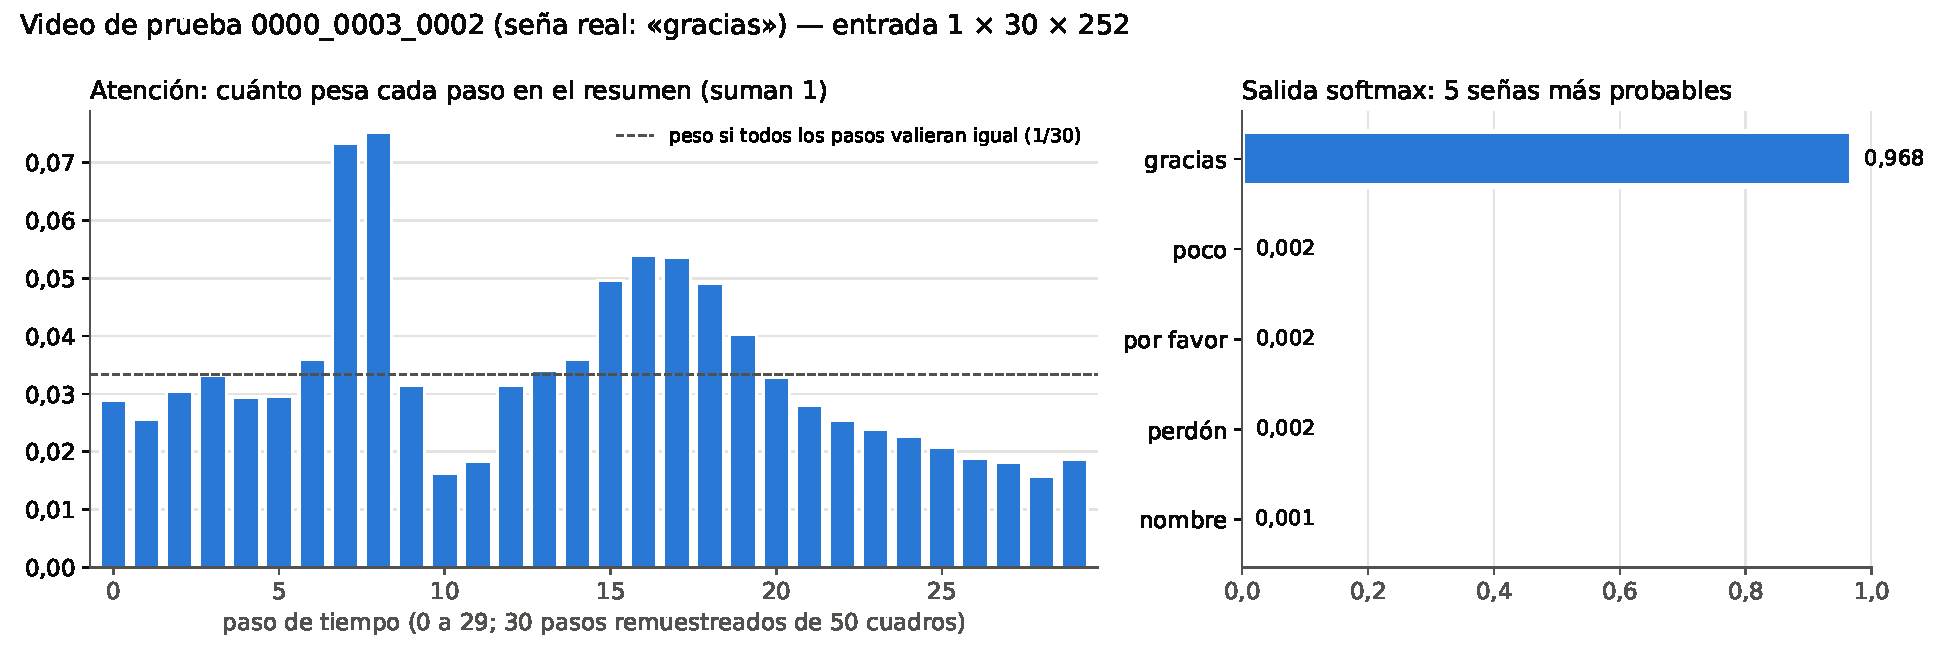
\includegraphics[width=\linewidth,height=3.6cm,keepaspectratio]{pasada_modelo_0000_0003_0002.pdf}

\vspace{0.02cm}
\scriptsize
Video 0000\_0003\_0002 («gracias», persona 0003): del conjunto de \textbf{prueba}; la red nunca lo vio, aunque sí a esa persona en otros videos. La atención pesa más en los pasos 7-8 y 15-18, contando de 0 a 29 (máximo 0,075 frente a 1/30 = 0,033); es un solo video y no se interpreta lingüísticamente. La probabilidad coincide con la guardada (0,96836).
\fuente{figuras/pasada\_modelo\_0000\_0003\_0002.json (formas, atencion con índices 0 a 29, top5); guion guiones/pasada\_modelo\_un\_video.py; models/canonico\_holistic\_mascara\_manos/evaluacion\_modelo\_seleccionado/predicciones.json.}
\end{frame}

% =====================================================================
\begin{frame}[fragile]{El prototipo arma exactamente la misma entrada que el entrenamiento}\label{fr:proto}
\begin{columns}[T]
\begin{column}{0.55\textwidth}
\small
\textbf{\color{azul}Tres comprobaciones} con las 3 muestras; en las tres la diferencia máxima es \textbf{0}:
\begin{enumerate}\setlength\itemsep{3pt}
  \item Los puntos extraídos hoy son los mismos que se guardaron del corpus.
  \item La fila normalizada es la misma que se usó para entrenar.
  \item El prototipo, alimentado con los cuadros del video y sus marcas de tiempo (sin cámara ni voz), arma la misma entrada y da las mismas 50 probabilidades.
\end{enumerate}
\medskip
\footnotesize
Con el reloj real y el video pasado más rápido que 24 fps, la confianza cambia entre corridas (en «con gusto», de 0,370 a 0,56-0,58 en las 3 corridas registradas), pero \textbf{la clase no cambió} en ninguna.
\end{column}
\begin{column}{0.42\textwidth}
\footnotesize
\textbf{\color{azul}Para repetirla} (desde la raíz del repositorio; $\approx$1-2 min; no abre la cámara ni suena):
\begin{tcolorbox}[colback=grisclaro,colframe=gris!40,boxrule=0.4pt,arc=1pt,left=2pt,right=2pt,top=1pt,bottom=1pt]
{\fontsize{7}{8.4}\selectfont
\begin{verbatim}
python docs/diapositivas_workflow/
  guiones/prueba_escritorio.py 0030_0000_0000
\end{verbatim}
}
\end{tcolorbox}
\scriptsize Otros comandos (la red por dentro, el prototipo en vivo) en A11 (pág.~\pageref{fr:comandos}).
\end{column}
\end{columns}
\fuente{figuras/prueba\_escritorio.json (extraccion.dif\_max\_vs\_extraccion\_guardada, entrenador.dif\_max, prototipo.reloj\_del\_video, prototipo.reloj\_real); reloj real de «con gusto» 0,5648 / 0,5728 / 0,5758: figuras/corridas\_reloj\_real/ (3 corridas del 30-sep-2026).}
\end{frame}

% =====================================================================
\section{Resultados}
\begin{frame}{Dos maneras de probar: personas nuevas y personas conocidas}\label{fr:esquemas}
\begin{columns}[c]
\begin{column}{0.57\textwidth}
\centering
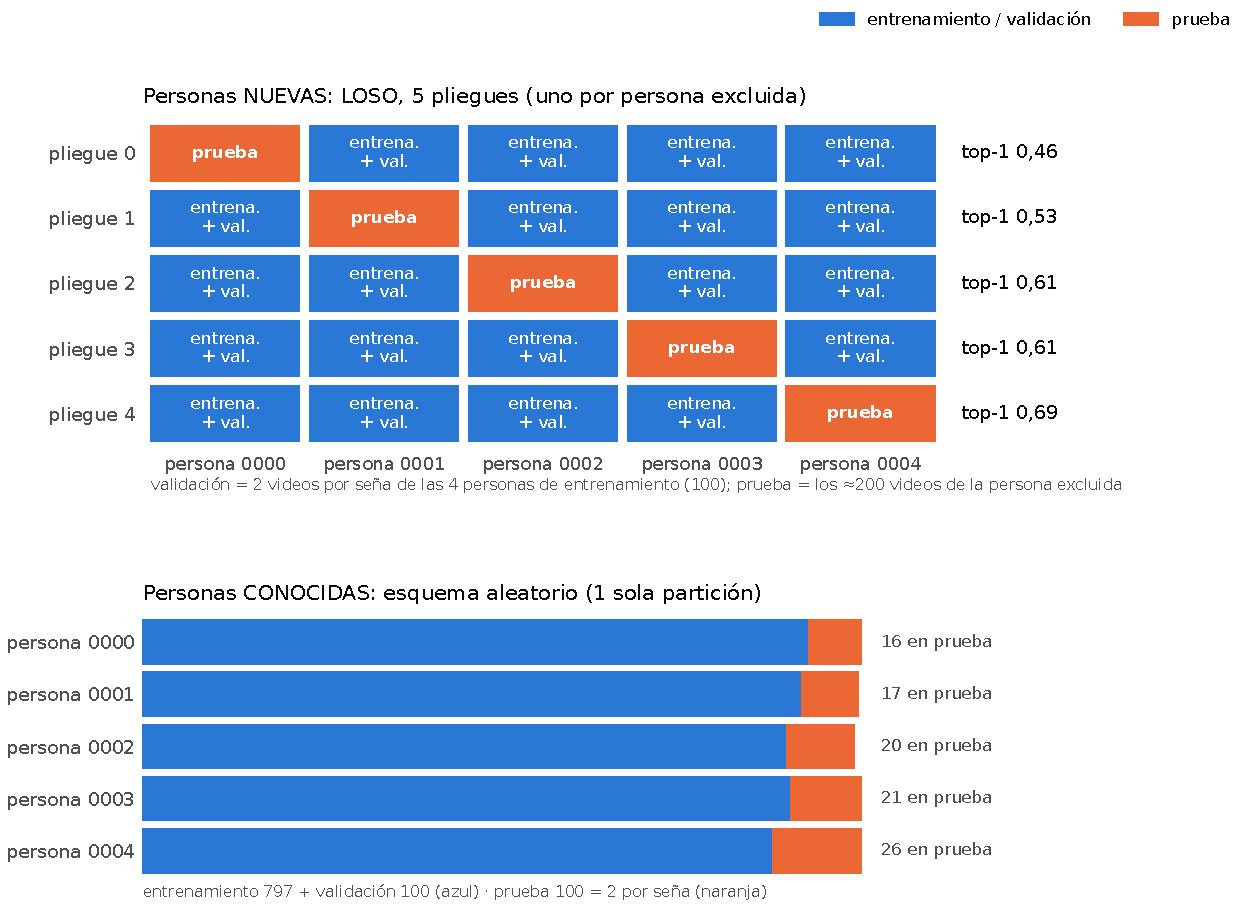
\includegraphics[width=\linewidth,height=6.1cm,keepaspectratio]{res_esquemas_particion.pdf}
\end{column}
\begin{column}{0.41\textwidth}
\begin{defi}[fontupper=\scriptsize]
\textbf{LOSO} (\emph{leave-one-signer-out}, dejar una persona fuera): se entrenan 5 modelos desde cero; cada uno se entrena con 4 personas (697-699 videos, 100 de validación) y se prueba con \textbf{todos} los videos de la quinta (198-200).
\end{defi}
\footnotesize
\begin{itemize}\setlength\itemsep{2pt}
  \item Es una validación cruzada de 5 pliegues: cada uno de los 997 videos se prueba una vez, con un modelo que no vio a esa persona.
  \item \textbf{Personas conocidas} (aleatorio): las 5 personas están en entrenamiento y en prueba (16-26 videos de cada una en prueba).
  \item La cifra principal es la de personas nuevas; la otra es un contraste optimista y no se restan.
\end{itemize}
\end{column}
\end{columns}
\fuente{models/loso\_2026-09-15\_holistic\_mascara\_manos/resultados\_loso.json (pliegues[k]); data/partitions/*.json; D-06; figura: guiones/figuras\_resultados.py (fig\_esquemas).}
\end{frame}

% =====================================================================
\begin{frame}{Cómo se mide: TP, FN y FP con la seña «hola»}\label{fr:metricas}
\begin{columns}[T]
\begin{column}{0.46\textwidth}
\scriptsize
\renewcommand{\arraystretch}{1.12}
\begin{tabularx}{\linewidth}{@{}>{\bfseries}l X@{}}
\toprule
Top-1 & exactitud (\emph{accuracy}): proporción de videos cuya seña más probable es la correcta. \\
Top-3 & la correcta está entre las 3 más probables. \\
TP & verdadero positivo: era «hola» y dijo «hola». \\
FN & falso negativo: era «hola» y dijo otra. \\
FP & falso positivo: dijo «hola» y era otra. \\
Recall & TP / (TP + FN): de las «hola» reales, cuántas reconoce. \\
Precisión & TP / (TP + FP): de las veces que dice «hola», cuántas acierta. \\
F1 & media armónica de precisión y recall. \\
Macro & se calcula por seña y se promedian las 50 por igual. \\
\bottomrule
\end{tabularx}
\end{column}
\begin{column}{0.52\textwidth}
\centering
\begin{tikzpicture}[
  c/.style={rounded corners=2pt,align=center,font=\sffamily\scriptsize,inner sep=3pt},
  fl/.style={-{Stealth[length=1.5mm]},thick,gris}]
  \node[c,draw=azul,fill=azulclaro!60,text width=3.0cm] (real) {\textbf{20 videos reales de «hola»}\\ (personas nuevas, LOSO)};
  \node[c,draw=verde,fill=verde!15,text width=1.9cm,below left=0.55cm and -1.1cm of real] (tp) {\textbf{TP = 10}\\ dijo «hola»};
  \node[c,draw=naranja,fill=naranja!15,text width=2.1cm,below right=0.55cm and -1.1cm of real] (fn) {\textbf{FN = 10}\\ 6 «hombre»\\ 4 «abuelo»};
  \draw[fl] (real) -- (tp); \draw[fl] (real) -- (fn);
  \node[c,draw=morado,fill=morado!10,text width=2.6cm,below=1.9cm of real,xshift=-0.6cm] (dijo) {\textbf{El modelo dijo «hola» 28 veces}};
  \node[c,draw=naranja,fill=naranja!15,text width=3.0cm,right=0.2cm of dijo] (fp) {\textbf{FP = 18}: 2 triste, 2 niño, 2 comer, 2 ¿cuándo?, 2 abuelo, 2 ¿quién?, 6 otras};
  \draw[fl] (dijo) -- (fp); \draw[fl] (dijo.north west) -- (tp.south);
\end{tikzpicture}

\vspace{0.1cm}
\footnotesize
Recall = 10/20 = \textbf{0,50} \quad Precisión = 10/28 = \textbf{0,357} \quad F1 = \textbf{0,417}\\[2pt]
\scriptsize Contraste: «buenos días» TP 20, FN 0, FP 0 (recall y precisión 1,00).
\end{column}
\end{columns}
\fuente{figuras/res\_metricas.json → ejemplo\_hola y por\_sena (desde models/loso\_2026-09-15\_holistic\_mascara\_manos/pliegue\_\{0..4\}/predicciones.json); guion guiones/resultados\_metricas.py.}
\end{frame}

% =====================================================================
\begin{frame}{Personas nuevas: 58 \% a la primera, 77 \% entre las tres primeras}\label{fr:nuevas}
\begin{columns}[c]
\begin{column}{0.52\textwidth}
\centering
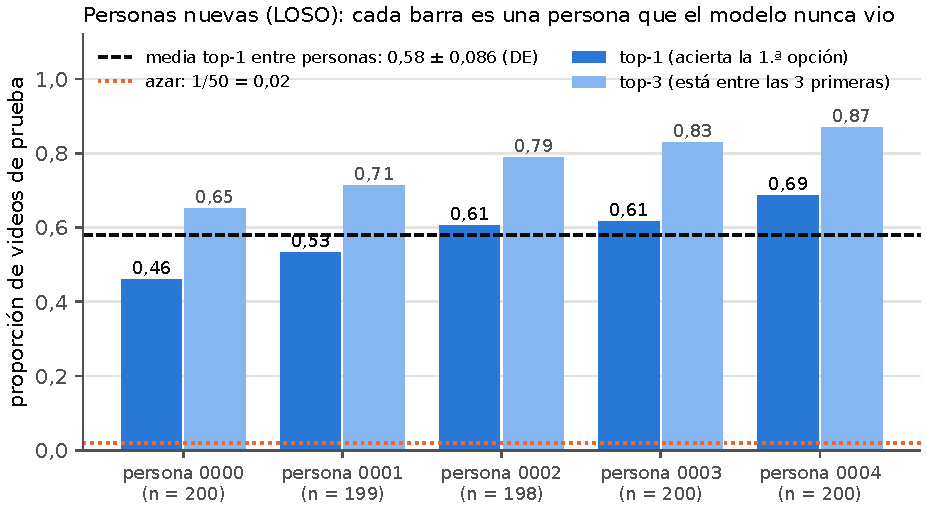
\includegraphics[width=\linewidth,height=5.2cm,keepaspectratio]{res_top1_por_persona.pdf}
\end{column}
\begin{column}{0.46\textwidth}
\scriptsize
\renewcommand{\arraystretch}{1.1}
\setlength\tabcolsep{4pt}
\begin{tabular}{@{}l r r r@{}}
\toprule
Persona nueva & Top-1 & Top-3 & F1 macro \\
\midrule
0000 (200 videos) & 0,460 & 0,650 & 0,421 \\
0001 (199) & 0,533 & 0,714 & 0,463 \\
0002 (198) & 0,606 & 0,788 & 0,573 \\
0003 (200) & 0,615 & 0,830 & 0,585 \\
0004 (200) & 0,685 & 0,870 & 0,645 \\
\midrule
\textbf{Media} & \textbf{0,580} & \textbf{0,770} & \textbf{0,537} \\
\textbf{DE entre personas} & 0,086 & 0,089 & 0,093 \\
\bottomrule
\end{tabular}\par\medskip
\footnotesize
\begin{itemize}\setlength\itemsep{1pt}
  \item Precisión macro 0,557 $\pm$ 0,088; recall macro 0,581 $\pm$ 0,086 (media entre personas).
  \item Sobre las 997 juntas: 578 aciertos y 419 errores; F1 macro \emph{agregado} 0,574.
  \item Con solo 5 personas la DE es una estimación gruesa.
\end{itemize}
\end{column}
\end{columns}
\fuente{models/loso\_2026-09-15\_holistic\_mascara\_manos/resultados\_loso.json (agregado; recalculado de pliegue\_k/predicciones.json en figuras/res\_metricas.json); N-30, N-35; F1: N-49 (media entre pliegues como cifra principal, pendiente de conformidad).}
\end{frame}

% =====================================================================
\begin{frame}{Personas conocidas: 0,88 en prueba, y resultado estable entre semillas}\label{fr:conocidas}
\begin{columns}[T]
\begin{column}{0.56\textwidth}
\scriptsize
\textbf{\color{azul}\small Prueba, esquema aleatorio (100 videos, 2 por seña)}\par\smallskip
\renewcommand{\arraystretch}{1.12}
\setlength\tabcolsep{3.5pt}
\begin{tabular}{@{}l r r r r r r@{}}
\toprule
Modelo & Top-1 & Top-3 & Prec. & Recall & F1 & Errores \\
\midrule
Semilla 2026 (prototipo) & \textbf{0,88} & 0,98 & 0,897 & 0,88 & 0,871 & 12 \\
5 semillas juntas & 0,91 & 1,00 & 0,93 & 0,91 & 0,909 & 9 \\
\bottomrule
\end{tabular}\par\bigskip
\textbf{\color{azul}\small Repetibilidad: validación de las 5 semillas (100 videos)}\par
{\color{gris}semilla = número que fija el azar del entrenamiento}\par\smallskip
\setlength\tabcolsep{3.5pt}
\begin{tabular}{@{}l r r r r r | r@{}}
\toprule
Semilla & 2026 & 2027 & 2028 & 2029 & 2030 & media $\pm$ DE \\
\midrule
Top-1 & 0,96 & 0,94 & 0,95 & 0,95 & 0,94 & 0,948 $\pm$ 0,008 \\
\bottomrule
\end{tabular}\par\smallskip
F1 de validación 0,945 $\pm$ 0,009; top-3 0,982 $\pm$ 0,008.
\end{column}
\begin{column}{0.42\textwidth}
\footnotesize
\begin{itemize}\setlength\itemsep{3pt}
  \item Los videos de prueba nunca se usaron para entrenar ni para elegir; pero sus personas sí aparecen en el entrenamiento.
  \item Con 100 videos que no vio, de personas que sí conoce, acierta 88.
  \item 100 videos: 1 punto = 1 video. No se compara restándolo del LOSO: son preguntas distintas.
  \item El prototipo usa un solo modelo (la semilla 2026); las 5 juntas son solo un contraste.
\end{itemize}
\end{column}
\end{columns}
\fuente{models/canonico\_holistic\_mascara\_manos/evaluacion\_modelo\_seleccionado/ y evaluacion\_ensemble/ (predicciones.json, metricas.json; recalculado en figuras/res\_metricas.json); resultados.json → semillas[]; N-31; docs/REPORTE\_COMPARATIVO\_4e.md §2.3.}
\end{frame}

% =====================================================================
\begin{frame}{Los errores no son al azar: se confunden señas parecidas}\label{fr:confusion}
\begin{columns}[c]
\begin{column}{0.5\textwidth}
\centering
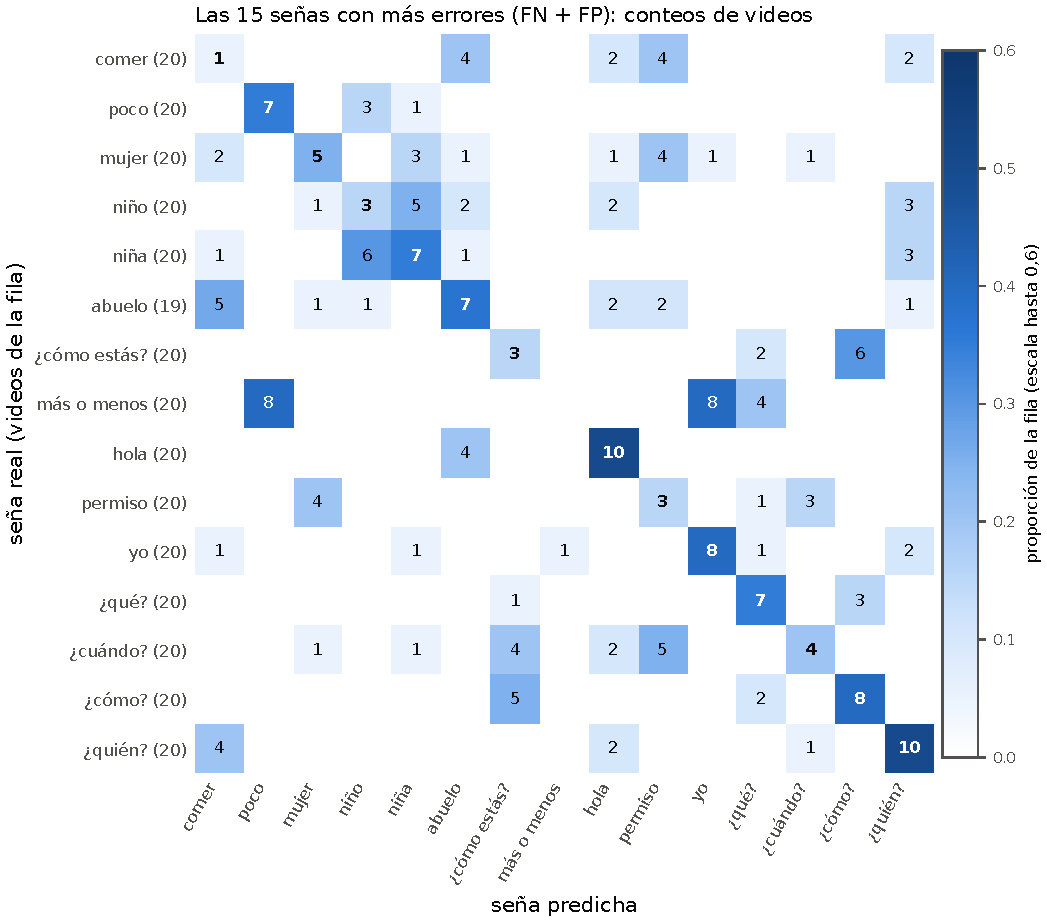
\includegraphics[width=\linewidth,height=6.1cm,keepaspectratio]{res_matriz_confusion_15.pdf}
\end{column}
\begin{column}{0.48\textwidth}
\begin{defi}[fontupper=\scriptsize]
\textbf{Matriz de confusión}: fila = seña real; columna = seña que dijo el modelo; diagonal = aciertos. Aquí, las 15 señas con más errores (FN + FP), en número de videos de personas nuevas.
\end{defi}
\footnotesize
\begin{itemize}\setlength\itemsep{2pt}
  \item «niño» $\leftrightarrow$ «niña»: 11 errores (5 y 6).
  \item «¿cómo estás?» $\leftrightarrow$ «¿cómo?»: 11 (6 y 5).
  \item «más o menos» nunca se acierta: 8 veces «poco», 8 «yo» y 4 «¿qué?».
  \item «comer» $\leftrightarrow$ «abuelo»: 9; «¿qué?» $\rightarrow$ «¿dónde?»: 6.
  \item El 29,6 \% de los 419 errores cae en la misma categoría gramatical (13,6 \% esperado al azar).
\end{itemize}
\scriptsize Solo muestra confusiones entre estas 15: las filas no suman 20. Matriz completa en el apéndice (pág.~\pageref{fr:m50}).
\end{column}
\end{columns}
\fuente{figuras/res\_metricas.json → matriz\_confusion\_997, pares\_no\_dirigidos\_top10, pares\_dirigidos\_top12; N-35 (models/analisis\_errores\_manos\_2026-09-15/analisis.json); figura: guiones/figuras\_resultados.py.}
\end{frame}

% =====================================================================
\begin{frame}{No todas las señas son igual de difíciles}\label{fr:porsena}
\begin{columns}[c]
\begin{column}{0.58\textwidth}
\centering
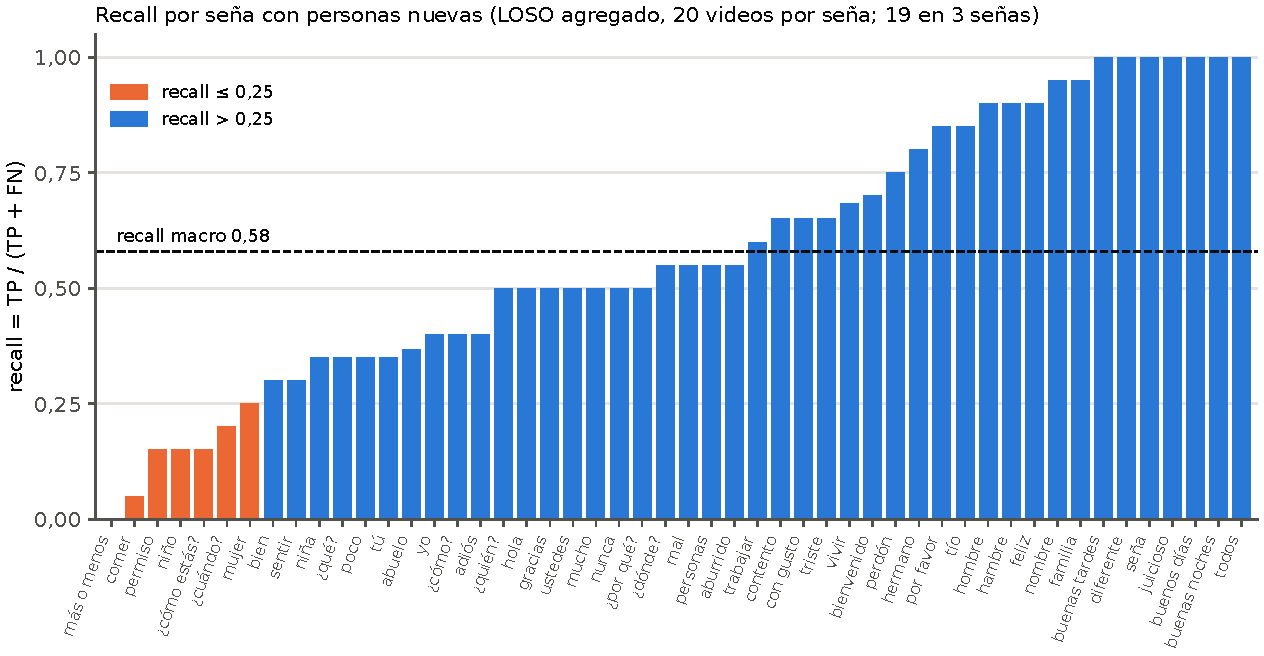
\includegraphics[width=\linewidth,height=5.3cm,keepaspectratio]{res_recall_por_sena.pdf}
\end{column}
\begin{column}{0.4\textwidth}
\footnotesize 15 de 50 señas alcanzan o superan 0,80 de recall (7 lo tienen de 1,00); 7 quedan en 0,25 o menos.\par\smallskip
\scriptsize
\renewcommand{\arraystretch}{1.05}
\begin{tabular}{@{}l r r r r@{}}
\toprule
Seña & TP & FN & FP & Recall \\
\midrule
\multicolumn{5}{@{}l}{\color{verde}\textbf{Mejores} (5 de las 7 con recall 1,00)}\\
buenos días & 20 & 0 & 0 & 1,00 \\
buenas noches & 20 & 0 & 0 & 1,00 \\
todos & 20 & 0 & 0 & 1,00 \\
seña & 20 & 0 & 2 & 1,00 \\
juicioso & 20 & 0 & 2 & 1,00 \\
\midrule
\multicolumn{5}{@{}l}{\color{naranja}\textbf{Peores}}\\
más o menos & 0 & 20 & 4 & 0,00 \\
comer & 1 & 19 & 18 & 0,05 \\
permiso & 3 & 17 & 23 & 0,15 \\
niño & 3 & 17 & 21 & 0,15 \\
¿cómo estás? & 3 & 17 & 17 & 0,15 \\
\bottomrule
\end{tabular}\par\smallskip
Recall por grupo: interrogativos 0,379; bien/mal/más o menos 0,283; emociones 0,688; resto 0,632.
\end{column}
\end{columns}
\fuente{figuras/res\_metricas.json → por\_sena, mejores\_5\_por\_recall, peores\_5\_por\_recall, senas\_recall\_ge\_0\_8, senas\_recall\_le\_0\_25; N-30, N-35. Tabla de las 50 señas en el apéndice (pág.~\pageref{fr:tabla1}).}
\end{frame}

% =====================================================================
\begin{frame}{¿Hace falta una red temporal? La línea base clásica acierta menos}\label{fr:lineabase}
\begin{columns}[c]
\begin{column}{0.55\textwidth}
\centering
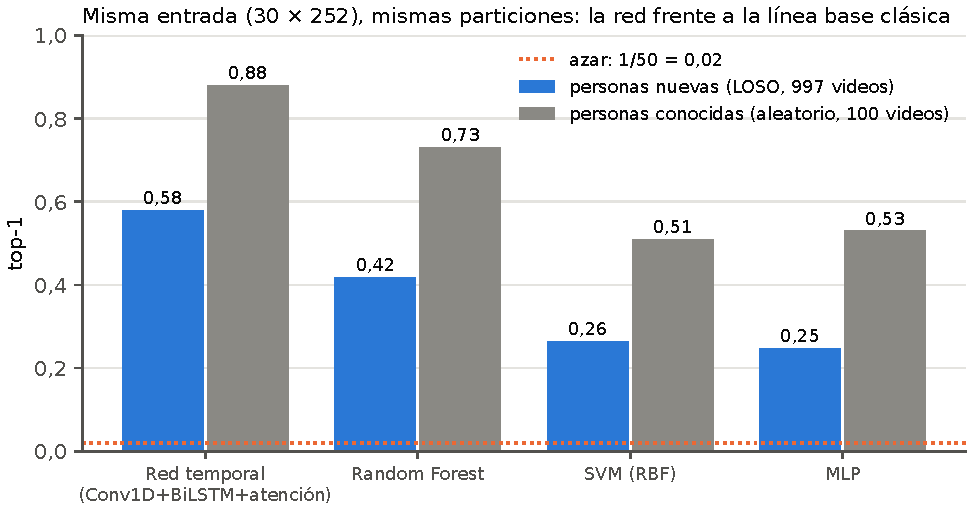
\includegraphics[width=\linewidth,height=5.2cm,keepaspectratio]{res_red_vs_linea_base.pdf}
\end{column}
\begin{column}{0.43\textwidth}
\footnotesize
\begin{itemize}\setlength\itemsep{3pt}
  \item Línea base: la misma matriz 30 $\times$ 252 resumida en 8 estadísticos por columna (2.016 números), \textbf{sin el orden temporal}, con las mismas particiones.
  \item Tres clasificadores clásicos (Random Forest, SVM y MLP). Personas nuevas: red 0,580; Random Forest 0,418; SVM 0,264; MLP 0,248.
  \item La diferencia red–Random Forest es significativa (McNemar, p = 2,9$\cdot$10$^{-18}$).
  \item Con la misma aumentación $\times$10, Random Forest solo sube a 0,442 (p = 3,0$\cdot$10$^{-15}$).
  \item Todos los sistemas bajan con personas nuevas (red 0,88 $\rightarrow$ 0,58; Random Forest 0,73 $\rightarrow$ 0,42): la brecha entre personas vistas y nuevas no es exclusiva de la red.
\end{itemize}
\end{column}
\end{columns}
\fuente{models/linea\_base\_4d\_2026-09-15/resultados.json (red.metricas\_agregadas, loso.con\_espejo.agregado\_997, aleatoria.con\_espejo.familias.random\_forest.prueba.top1, comparacion\_mcnemar) y control\_aumentacion\_completa/; D-10, N-39 (actividades 2.c/2.d según D-11); figura: guiones/figuras\_resultados.py.}
\end{frame}

% =====================================================================
\begin{frame}{Desempeño: la máquina responde en 36 ms; la espera es la ventana}\label{fr:latencia}
\begin{columns}[T]
\begin{column}{0.62\textwidth}
\scriptsize
\renewcommand{\arraystretch}{1.1}
\begin{tabularx}{\linewidth}{@{}>{\raggedright\arraybackslash\hyphenpenalty=10000\exhyphenpenalty=10000}X r r@{}}
\toprule
Etapa (sesiones del 22-sep, cámara integrada) & Tiempo & n \\
\midrule
Captura: ventana (74,9 cuadros a 30,4 fps) & 2.484 ms & 10 ventanas \\
Extracción MediaPipe, durante la captura & 12,2 ms/cuadro & 749 cuadros \\
Preprocesamiento (normalizar, 30 pasos, velocidades) & 0,5 ms & 10 \\
Inferencia de la red & 21,9 ms & 10 \\
Conversión a español & 0,0 ms & 3 \\
Síntesis de voz (frase ya guardada) & 0,5 ms & 3 \\
\quad frase nueva, no guardada & 22,0 ms & 1 \\
\midrule
\textbf{Respuesta}: cierre de la ventana $\rightarrow$ orden de reproducir la voz & \textbf{36,4 ms} (35,1-37,2) & 3 \\
\textbf{Total}: apertura de la ventana $\rightarrow$ orden de reproducir la voz & \textbf{2.521 ms} & 3 \\
\bottomrule
\end{tabularx}
\end{column}
\begin{column}{0.36\textwidth}
\footnotesize
\begin{itemize}\setlength\itemsep{3pt}
  \item Equipo: Apple M5 Max, 18 núcleos, 48 GB; \textbf{solo CPU}.
  \item 12,2 ms por cuadro cabe en el tiempo entre cuadros ($\approx$32,9 ms a 30,4 fps).
  \item n muy pequeño: confirma el funcionamiento; las cifras finales se medirán en la prueba formal.
  \item Con todos los registros en vivo (14, 15 y 22-sep; incluye sesiones con el modelo anterior de 225 rasgos): extracción 12,1 ms (n = 5.951 cuadros), inferencia 20,2 ms (n = 77).
\end{itemize}
\end{column}
\end{columns}
\fuente{src/latencia\_resumen.py sobre registros/latencia\_2026-09-22.jsonl $\rightarrow$ figuras/res\_latencia\_2026-09-22.json; N-52 (frase nueva 22,0 ms); todos los registros: src/latencia\_resumen.py sobre registros/latencia\_2026-09-14, -15 y -22.jsonl (N-26, N-32); equipo: N-21 y resultados\_loso.json → entorno; README.md l. 732 (la marca final es la orden de reproducción, no el sonido).}
\end{frame}

% =====================================================================
\section{De los datos a la prueba real}
\begin{frame}{Umbral: cuándo el sistema pide que se repita la seña}\label{fr:umbral}
\flujo{8}
\begin{columns}[c]
\begin{column}{0.47\textwidth}
\centering
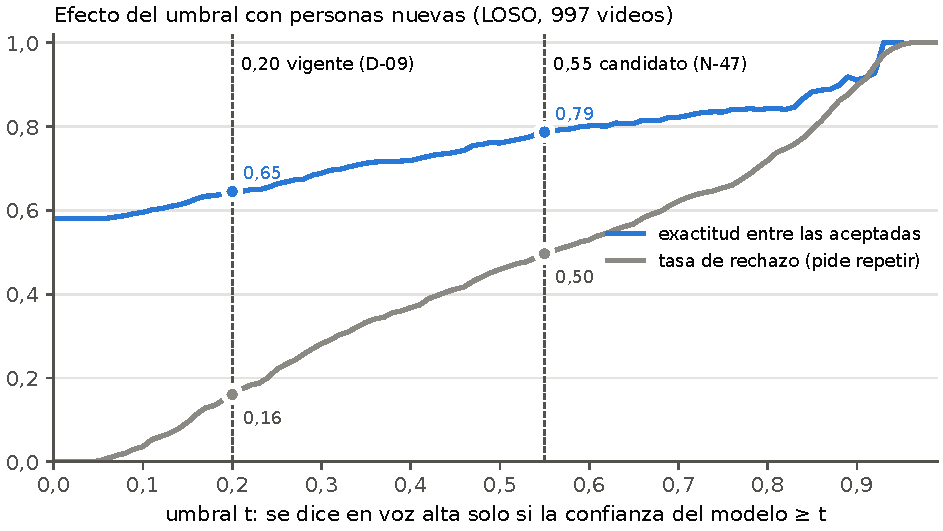
\includegraphics[width=\linewidth,height=5.1cm,keepaspectratio]{res_umbral.pdf}
\end{column}
\begin{column}{0.51\textwidth}
\footnotesize 0,20 es el vigente; 0,55, el propuesto.\par\smallskip
\scriptsize
Personas nuevas (LOSO, 997 videos):\par\smallskip
\renewcommand{\arraystretch}{1.1}
\setlength\tabcolsep{3.5pt}
\begin{tabular}{@{}l r r r@{}}
\toprule
Umbral & Rechazo & Exactitud & Dichas \\
 & & (aceptadas) & mal \\
\midrule
0,20 (vigente) & 16,0 \% & 0,645 & 297 \\
0,55 global (candidato) & 49,6 \% & 0,787 & 107 \\
uno por pliegue (0,48-0,67) & 52,3 \% & 0,782 & 104 \\
\bottomrule
\end{tabular}\par\medskip
\scriptsize
\begin{itemize}\setlength\itemsep{2pt}
  \item Con el umbral elegido por pliegue (cifra limpia) se dicen 193 señas equivocadas menos a cambio de 168 aciertos menos (con 0,55 global: 190 y 145), y se pide repetir la mitad de las veces.
  \item Utilidad U = aciertos dichos $-$ errores dichos: 243 con 0,20; 268 por pliegue. La ganancia en utilidad (+25) no es concluyente: intervalo de confianza del 95 \% de $-$12 a +62.
  \item El top-1 y el top-3 no dependen del umbral. \textbf{Lo decide el director.}
\end{itemize}
\end{column}
\end{columns}
\fuente{figuras/res\_metricas.json → umbral (0,20 y 0,55: aceptadas\_correctas / aceptadas\_incorrectas); models/umbral\_anidado\_2026-09-22/resultados\_anidado.json → efecto\_prueba\_loso, control\_N33, seleccion (U con c = 1); N-47 (umbrales por pliegue 0,50 / 0,66 / 0,67 / 0,58 / 0,48; IC por bootstrap); D-09, N-33, N-51.}
\end{frame}

% =====================================================================
\begin{frame}{Condiciones de captura: hoy el prototipo en vivo no replica las del corpus}\label{fr:condiciones}
\fontsize{6.4}{7.5}\selectfont
\renewcommand{\arraystretch}{1.08}
\begin{tabularx}{\textwidth}{@{}>{\bfseries\raggedright\arraybackslash}p{1.45cm} >{\raggedright\arraybackslash\leavevmode}X >{\raggedright\arraybackslash\leavevmode}X >{\raggedright\arraybackslash\leavevmode}X >{\centering\arraybackslash}p{0.95cm}@{}}
\toprule
Condición & Corpus LSC50 (\texttt{COLOR\_BODY}) & Prototipo en vivo hasta hoy & \textbf{Propuesta} para la prueba formal (sin adoptar) & ¿Igual hoy? \\
\midrule
Cámara & Kinect V2 RGB en trípode & cámara integrada del portátil & webcam externa Full HD en trípode & no \\
Resolución & 1920$\times$1080 & 640$\times$480 pedida; la efectiva sale en consola, no en el registro & 1920$\times$1080 si la tasa no cae más de 10 \% & no \\
Tasa & 24 fps & 30,4 fps medidos & la del piloto & no* \\
Distancia & 200 cm & no registrada & 200 cm, marca en el piso & sin dato \\
Encuadre & rodillas a brazos extendidos & no registrado & igual al del corpus & sin dato \\
Fondo & cortina azul 3 $\times$ 3 m, a 10 cm & no registrado & liso y uniforme (sin cortina) & parcial \\
Iluminación & blanca y homogénea & no registrada & luz artificial constante, persianas cerradas, luz medida & parcial \\
Oclusión & no registrada; manos detectadas: izq. 93,8 \%, der. 97,2 \% de los cuadros; ninguna, 0,44 \% & se guarda por ventana la proporción de cuadros sin ninguna mano (22-sep: 0 a 0,41); no la causa & caso límite a provocar (ocultar una mano): se infiere con esa mano en 0 & sin dato \\
Desenfoque & no medido & no medido & no está en la propuesta & sin dato \\
Persona & 5 personas fluidas en LSC & el autor, sin LSC, fuera del corpus & profesor de LSC vinculado (LSC), que aceptó ayudar & no \\
Inicio y fin & empieza en movimiento, termina en reposo & ESPACIO abre 2,5 s = 75 cuadros & reposo al abrir y al cerrar & parcial \\
Normalización & por hombros & la misma & la misma & sí \\
\bottomrule
\end{tabularx}

\vspace{0.05cm}
{\fontsize{6.4}{7.5}\selectfont
Distancia, fondo, luz y encuadre del corpus son lo que \emph{declara} el artículo (no se verificaron mirando cuadros). *El remuestreo a 30 pasos iguala el número de pasos; su efecto no se ha medido.\par}
\fuente{caracterizacion.md §6, §8, §9; src/realtime.py l. 308, 330-331, 355-364; N-21 (detección en el corpus); registros/latencia\_2026-09-22.jsonl (proporcion\_sin\_manos); docs/PROTOCOLO\_EXPERIMENTAL\_4a.md §5.3 (CL-3); docs/PROPUESTA\_PARAMETROS\_4a.md l. 41, 95-97 (PD-06 a PD-08, PD-10); N-26, N-32, N-48, N-50, N-52, N-54; anteproyecto 09\_metodologia.tex l. 274-276 y 498-502 (hay que documentar estas diferencias).}
\end{frame}

% =====================================================================
\begin{frame}{Estado: modelo y prototipo listos; falta la prueba formal en vivo}\label{fr:estado}
\begin{columns}[T]
\begin{column}{0.325\textwidth}
\begin{tcolorbox}[colback=verde!8,colframe=verde,title=\textbf{Hecho},fonttitle=\small,fontupper=\scriptsize,arc=1pt,boxrule=0.6pt,left=3pt,right=3pt,top=2pt,bottom=2pt]
\begin{itemize}\setlength\itemsep{1pt}\setlength\leftmargini{1em}
  \item Integridad del corpus {\color{gris}(1.a)}
  \item Caracterización del corpus {\color{gris}(1.b)}
  \item Extracción propia de puntos y su tasa {\color{gris}(1.c)}
  \item Particiones de los datos {\color{gris}(1.e)}
  \item Representación de entrada: solo manos {\color{gris}(2.a)}
  \item Entrenamiento, línea base y selección del modelo {\color{gris}(2.c, 2.d)}
  \item Voz local, sin internet {\color{gris}(3.b)}
  \item Prototipo completo en vivo {\color{gris}(3.c)}
  \item Análisis de errores {\color{gris}(4.d)}
\end{itemize}
\end{tcolorbox}
\end{column}
\begin{column}{0.325\textwidth}
\begin{tcolorbox}[colback=naranja!8,colframe=naranja,title=\textbf{En curso o en borrador},fonttitle=\small,fontupper=\scriptsize,arc=1pt,boxrule=0.6pt,left=3pt,right=3pt,top=2pt,bottom=2pt]
\begin{itemize}\setlength\itemsep{1pt}
  \item Protocolo de la prueba en vivo: borrador y propuesta de parámetros, pendiente del director {\color{gris}(4.a)}
  \item Reporte comparativo de los dos esquemas: borrador {\color{gris}(4.e)}
  \item Consulta al registro de intérpretes (INSOR): radicada el 15-sep, sin respuesta {\color{gris}(0.b)}
  \item Persona señante: el profesor de LSC vinculado aceptó el 28-sep; faltan perfil, consentimiento escrito y comité de ética {\color{gris}(0.c)}
\end{itemize}
\end{tcolorbox}
\end{column}
\begin{column}{0.325\textwidth}
\begin{tcolorbox}[colback=grisclaro,colframe=gris,title=\textbf{Pendiente},fonttitle=\small,fontupper=\scriptsize,arc=1pt,boxrule=0.6pt,left=3pt,right=3pt,top=2pt,bottom=2pt]
\begin{itemize}\setlength\itemsep{1pt}
  \item Validación de los nombres de las 50 señas con el profesor de LSC vinculado {\color{gris}(1.d)}
  \item Rediseño de la conversión a español {\color{gris}(3.a)}
  \item Prueba en vivo con persona señante; exactitud y latencia formales {\color{gris}(4.b, 4.c)}
  \item Redacción del informe final
\end{itemize}
\smallskip
{\raggedright\hyphenpenalty=10000\textbf{Plazo} (según lo entendido por el estudiante; sin confirmación oficial): documento listo la 1.ª-2.ª semana de noviembre; sustentación a finales de noviembre.\par}
\end{tcolorbox}
\end{column}
\end{columns}
\fuente{anteproyecto 11\_cronograma.tex (nombres y códigos de actividad, en gris); DECISIONES\_TESIS.txt: hecho N-43, caracterizacion.md, N-21, N-40, D-06, D-08, N-30, N-31, N-39, D-11, N-45, N-26, N-32, N-52, N-35; en curso N-37, N-48, N-44, N-27, N-54; README.md (3.a, mes 3); plazos: reunión del 28-sep-2026 (transcripción, 21:43).}
\end{frame}

% =====================================================================
\begin{frame}{Decisiones pendientes con el director}\label{fr:decisiones}
\footnotesize
\renewcommand{\arraystretch}{1.18}
\begin{tabularx}{\textwidth}{@{}>{\leavevmode\color{azul}\bfseries\raggedright}p{2.6cm} >{\raggedright\arraybackslash\leavevmode}X >{\raggedright\arraybackslash}p{2.1cm}@{}}
\toprule
Decisión & Opciones y datos & Fuente \\
\midrule
Umbral de confianza & 0,20 vigente (16 \% de rechazo, 297 dichas mal) o 0,55 (50 \%, 107 dichas mal) & D-09, N-47 \\
Duración de la ventana & 2,5 s (cabe el 29,1 \% de los videos) o 3,0 s (68,0 \%) & N-48 (PD-09) \\
Qué F1 se reporta & principal: media entre pliegues 0,537 $\pm$ 0,093; complemento: agregado 0,574 & N-49 \\
Señas cortadas & propuesta: pedir reposo al abrir y cerrar la ventana y avisar sin rechazar & N-50 (PD-10) \\
Validación controlada con el profesor de LSC vinculado & sesión acotada: 4 repeticiones por seña (200 presentaciones, el tamaño de un pliegue LOSO) en dos sesiones de $\approx$58 min (estimado); captura cercana a la del corpus (cámara externa Full HD a 200 cm); máx. 2 intentos; cifra principal: top-1/top-3 del primer intento (también se reportan «todos los intentos» y «último intento») & N-48 \\
Persona señante & comité de ética, consentimiento escrito, perfil a declarar, reconocimiento económico & N-54 \\
\bottomrule
\end{tabularx}

\vspace{0.2cm}
\begin{clave}[fontupper=\footnotesize]
Hasta la respuesta del director no se adopta el umbral 0,55, ni los valores del protocolo, ni la propuesta para las señas cortadas.
\end{clave}
\fuente{DECISIONES\_TESIS.txt D-09, N-47, N-48, N-49, N-50, N-51 y N-54; docs/PROPUESTA\_PARAMETROS\_4a.md.}
\end{frame}

% =====================================================================
\appendix
\section{Apéndice}
\begin{frame}[plain]
\centering
\vspace{2.8cm}
{\Large\bfseries\color{azul}Apéndice}\par\medskip
{\small\color{gris}Tabla de capas · hiperparámetros · por qué solo manos · tabla por seña · matriz completa · duración por persona · otros hallazgos del EDA · glosario · comandos}
\end{frame}

% =====================================================================
\begin{frame}{A1. Tabla de capas del modelo canónico (formas sin el lote)}\label{fr:capas}
\fontsize{6.8}{8}\selectfont
\renewcommand{\arraystretch}{1.02}
\begin{columns}[T]
\begin{column}{0.5\textwidth}
\begin{tabular}{@{}l l r@{}}
\toprule
Capa & Salida & Parámetros \\
\midrule
Entrada & 30 $\times$ 252 & 0 \\
Conv1D 128 filtros, k = 3, \emph{same} & 30 $\times$ 128 & 96.896 \\
BatchNormalization & 30 $\times$ 128 & 256 / 256 \\
ReLU & 30 $\times$ 128 & 0 \\
Conv1D 128, k = 3 & 30 $\times$ 128 & 49.280 \\
BatchNormalization + ReLU & 30 $\times$ 128 & 256 / 256 \\
Dropout 0,15 & 30 $\times$ 128 & 0 \\
BiLSTM 128 + 128 (concat.) & 30 $\times$ 256 & 263.168 \\
BatchNormalization & 30 $\times$ 256 & 512 / 512 \\
Dropout 0,3 & 30 $\times$ 256 & 0 \\
BiLSTM 64 + 64 & 30 $\times$ 128 & 164.352 \\
BatchNormalization & 30 $\times$ 128 & 256 / 256 \\
Dropout 0,3 & 30 $\times$ 128 & 0 \\
\bottomrule
\end{tabular}
\end{column}
\begin{column}{0.48\textwidth}
\begin{tabular}{@{}l l r@{}}
\toprule
Capa & Salida & Parámetros \\
\midrule
Atención: Dense(1) lineal & 30 $\times$ 1 & 129 \\
\quad softmax sobre los 30 pasos & 30 $\times$ 1 & 0 \\
\quad multiplicar y promediar & 128 & 0 \\
Promedio en el tiempo & 128 & 0 \\
Máximo en el tiempo & 128 & 0 \\
Concatenar & 384 & 0 \\
Dense 256 ReLU & 256 & 98.560 \\
Dropout 0,3 & 256 & 0 \\
Dense 128 ReLU & 128 & 32.896 \\
Dropout 0,15 & 128 & 0 \\
Dense 50 softmax & 50 & 6.450 \\
\midrule
\textbf{Total} & & \textbf{713.011} + 1.280 \\
\bottomrule
\end{tabular}\par\medskip
En BatchNormalization: entrenables / no entrenables (medias y varianzas móviles). Total 714.291. Atención exacta: $\frac{1}{30}\sum_t \alpha_t x_t$ (el factor 1/30 lo absorbe la capa siguiente).
\end{column}
\end{columns}
\fuente{figuras/tabla\_capas\_modelo.json (generado cargando models/canonico\_holistic\_mascara\_manos/modelo\_canonico.keras; coincide con build\_model(30, 252, 50)); guion guiones/tabla\_capas\_modelo.py.}
\end{frame}

% =====================================================================
\begin{frame}{A2. Hiperparámetros exactos y aumentación}\label{fr:hiper}
\begin{columns}[T]
\begin{column}{0.49\textwidth}
\scriptsize\hyphenpenalty=10000
\renewcommand{\arraystretch}{1.1}
\begin{tabular}{@{}l >{\raggedright\arraybackslash}p{4.3cm}@{}}
\toprule
Optimizador & Adam ($\beta_1$ 0,9; $\beta_2$ 0,999; $\varepsilon$ 10$^{-7}$) \\
Tasa de aprendizaje & CosineDecay: inicial 0,001; 25.000 pasos (200 épocas $\times$ 125); $\alpha$ 10$^{-6}$; sin calentamiento \\
\quad en la práctica & 0,001 $\rightarrow$ 0,000982 (época 17) $\rightarrow$ 0,000895 (época 42) \\
Pérdida & entropía cruzada categórica, suavizado 0,1 (objetivo 0,902 / 0,002); mínimo posible 0,702 \\
Lote & 64 \\
Épocas & máx. 200; EarlyStopping sobre val\_accuracy, paciencia 25, restaura mejores pesos \\
Checkpoint & mejor val\_accuracy; guardado en la época 17 (2.125 iteraciones = 17 $\times$ 125) \\
Dropout base & 0,3 \\
Semillas & 2026-2030; empate: menor val\_loss \\
LOSO & misma arquitectura y ajustes; semilla 2026 \\
\bottomrule
\end{tabular}
\end{column}
\begin{column}{0.49\textwidth}
\scriptsize\hyphenpenalty=10000\raggedright
\renewcommand{\arraystretch}{1.1}
\begin{tabular}{@{}r l@{}}
\toprule
\# & Copia (antes de calcular velocidades) \\
\midrule
0 & original \\
1 & espejo: niega x e intercambia manos \\
2-4 & ruido gaussiano $\sigma$ 0,005 / 0,012 / 0,020 \\
5 & re-muestreo temporal, factor U(0,85-0,95) \\
6 & re-muestreo temporal, factor U(1,05-1,15) \\
7 & escala U(0,85-1,15) por muestra \\
8 & espejo + ruido $\sigma$ 0,008 \\
9 & espejo + re-muestreo U(0,9-1,1) \\
\bottomrule
\end{tabular}\par\medskip
El «re-muestreo temporal» no cambia la duración de la seña: conserva el primer y el último paso y re-interpola los 30 pasos por puntos intermedios.
\end{column}
\end{columns}
\fuente{src/train\_final\_100.py (l. 207-241, 425-451); src/train\_lstm.py; src/representacion.py (espejar); modelo\_canonico.keras (optimizer.get\_config, iterations); figuras/curvas\_aprendizaje\_semilla2026.json; resultados.json → configuracion, seleccion.}
\end{frame}

% =====================================================================
\begin{frame}{A3. ¿Por qué solo las manos? ¿Por qué coordenadas y no la imagen?}\label{fr:porque}
\centering
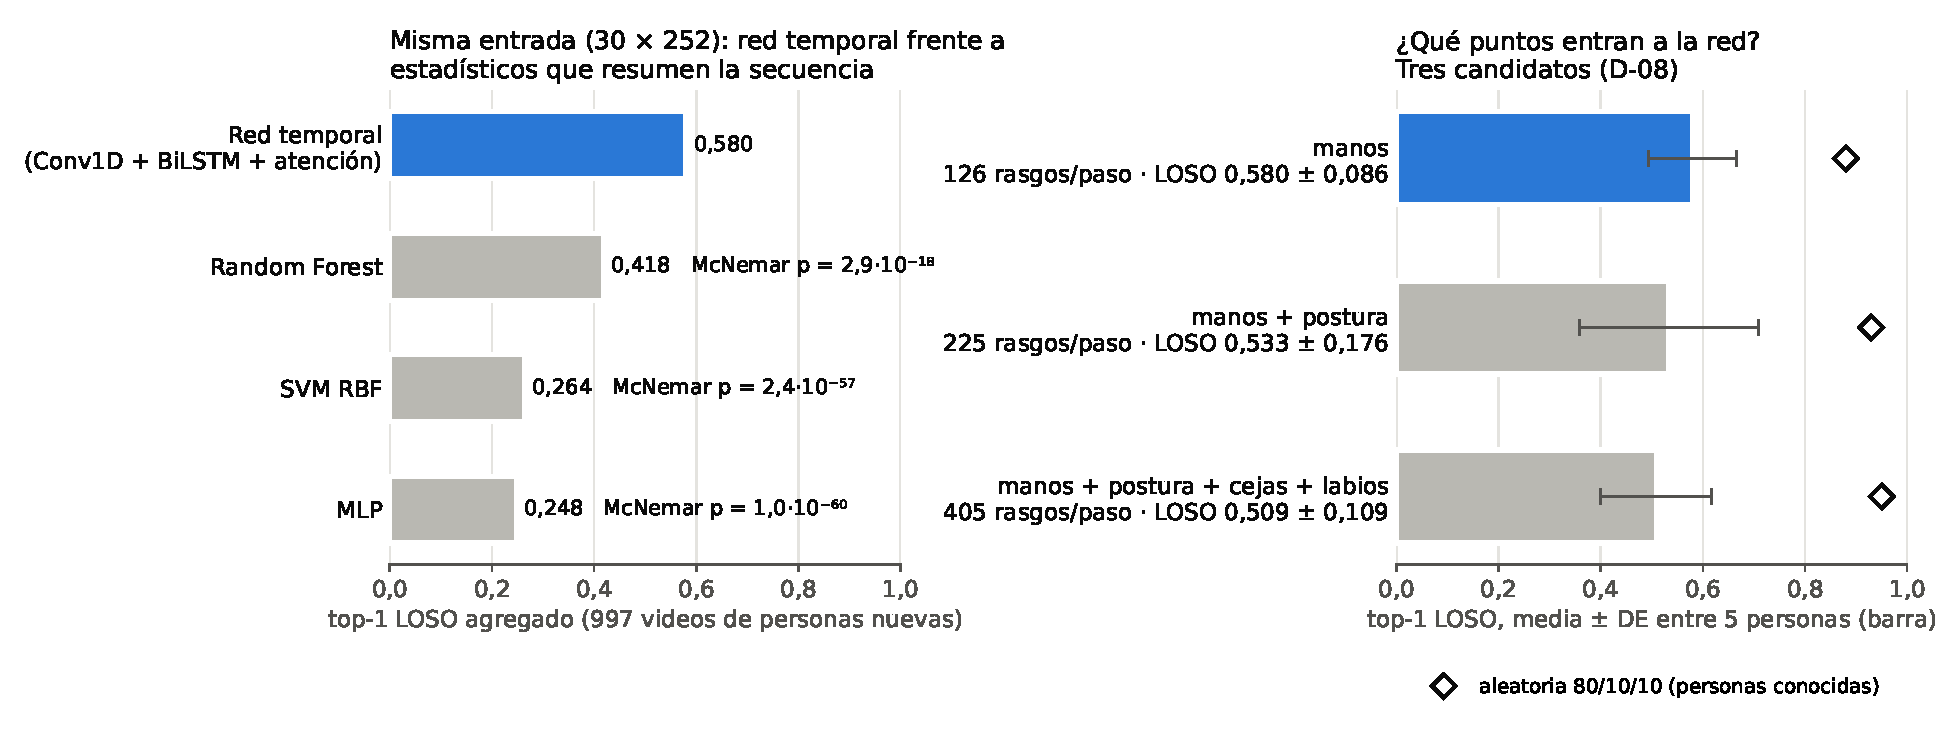
\includegraphics[width=\linewidth,height=4.2cm,keepaspectratio]{comparacion_red_y_representacion.pdf}

\vspace{0.05cm}
\begin{columns}[T]
\begin{column}{0.49\textwidth}
\scriptsize
\textbf{Qué puntos entran} (elegido por validación, criterio fijado antes): manos 126 rasgos $\rightarrow$ LOSO 0,580 $\pm$ 0,086; + postura (225) 0,533 $\pm$ 0,176; + cejas y labios (405) 0,509 $\pm$ 0,109. Con personas conocidas el orden se invierte (0,88 / 0,93 / 0,95).
\end{column}
\begin{column}{0.49\textwidth}
\scriptsize
\textbf{Coordenadas y no píxeles}: no hay experimento propio con píxeles. Razones: el requisito de CPU del anteproyecto y la evidencia externa en otro corpus (LSC70): 75,9 \% con la imagen de la mano frente a 87,6 \% con coordenadas de MediaPipe. No es una comparación homogénea con LSC50.
\end{column}
\end{columns}
\fuente{models/comparacion\_D08\_2026-09-15.json; D-08, N-30; N-39; anteproyecto 06\_alcances.tex:27-28 y 08\_marco.tex:415-418 (ref42); figura: guiones/comparacion\_red\_y\_representacion.py.}
\end{frame}

% =====================================================================
\begin{frame}{A4. Resultados por seña con personas nuevas (1 de 2): señas 0 a 24}\label{fr:tabla1}
\centering
\fontsize{6.6}{7.4}\selectfont
\renewcommand{\arraystretch}{0.9}
% Generado por docs/diapositivas_workflow/guiones/tabla_por_sena.py desde figuras/res_metricas.json:por_sena (LOSO agregado, 997).
\begin{tabular}{@{}r l r r r r r r@{}}
\toprule
ID & Seña & Videos & TP & FN & FP & Recall & Precisión \\
\midrule
0 & gracias & 20 & 10 & 10 & 10 & 0,50 & 0,50 \\
\rowcolor{verde!15}1 & buenos días & 20 & 20 & 0 & 0 & 1,00 & 1,00 \\
\rowcolor{verde!15}2 & buenas tardes & 19 & 19 & 0 & 9 & 1,00 & 0,68 \\
\rowcolor{verde!15}3 & buenas noches & 20 & 20 & 0 & 0 & 1,00 & 1,00 \\
\rowcolor{verde!15}4 & seña & 20 & 20 & 0 & 2 & 1,00 & 0,91 \\
\rowcolor{verde!15}5 & nombre & 20 & 19 & 1 & 2 & 0,95 & 0,90 \\
6 & trabajar & 20 & 12 & 8 & 0 & 0,60 & 1,00 \\
\rowcolor{naranja!15}7 & comer & 20 & 1 & 19 & 18 & 0,05 & 0,05 \\
8 & vivir & 19 & 13 & 6 & 15 & 0,68 & 0,46 \\
9 & poco & 20 & 7 & 13 & 9 & 0,35 & 0,44 \\
\rowcolor{verde!15}10 & familia & 20 & 19 & 1 & 1 & 0,95 & 0,95 \\
11 & personas & 20 & 11 & 9 & 5 & 0,55 & 0,69 \\
\rowcolor{naranja!15}12 & mujer & 20 & 5 & 15 & 10 & 0,25 & 0,33 \\
\rowcolor{verde!15}13 & hombre & 20 & 18 & 2 & 18 & 0,90 & 0,50 \\
\rowcolor{naranja!15}14 & niño & 20 & 3 & 17 & 21 & 0,15 & 0,12 \\
15 & niña & 20 & 7 & 13 & 19 & 0,35 & 0,27 \\
16 & abuelo & 19 & 7 & 12 & 19 & 0,37 & 0,27 \\
\rowcolor{verde!15}17 & tío & 20 & 17 & 3 & 5 & 0,85 & 0,77 \\
\rowcolor{verde!15}18 & hermano & 20 & 16 & 4 & 3 & 0,80 & 0,84 \\
\rowcolor{verde!15}19 & hambre & 20 & 18 & 2 & 6 & 0,90 & 0,75 \\
\rowcolor{verde!15}20 & feliz & 20 & 18 & 2 & 6 & 0,90 & 0,75 \\
21 & contento & 20 & 13 & 7 & 6 & 0,65 & 0,68 \\
22 & triste & 20 & 13 & 7 & 2 & 0,65 & 0,87 \\
23 & aburrido & 20 & 11 & 9 & 5 & 0,55 & 0,69 \\
24 & bien & 20 & 6 & 14 & 4 & 0,30 & 0,60 \\
\bottomrule
\end{tabular}

\fuente{figuras/res\_metricas.json → por\_sena (LOSO agregado, 997 predicciones); guion guiones/tabla\_por\_sena.py. Verde: recall $\geq$ 0,80; naranja: recall $\leq$ 0,25.}
\end{frame}

\begin{frame}{A5. Resultados por seña con personas nuevas (2 de 2): señas 25 a 49}\label{fr:tabla2}
\centering
\fontsize{6.6}{7.4}\selectfont
\renewcommand{\arraystretch}{0.9}
% Generado por docs/diapositivas_workflow/guiones/tabla_por_sena.py desde figuras/res_metricas.json:por_sena (LOSO agregado, 997).
\begin{tabular}{@{}r l r r r r r r@{}}
\toprule
ID & Seña & Videos & TP & FN & FP & Recall & Precisión \\
\midrule
25 & mal & 20 & 11 & 9 & 8 & 0,55 & 0,58 \\
\rowcolor{naranja!15}26 & ¿cómo estás? & 20 & 3 & 17 & 17 & 0,15 & 0,15 \\
\rowcolor{naranja!15}27 & más o menos & 20 & 0 & 20 & 4 & 0,00 & 0,00 \\
28 & sentir & 20 & 6 & 14 & 1 & 0,30 & 0,86 \\
\rowcolor{verde!15}29 & juicioso & 20 & 20 & 0 & 2 & 1,00 & 0,91 \\
30 & hola & 20 & 10 & 10 & 18 & 0,50 & 0,36 \\
31 & adiós & 20 & 8 & 12 & 6 & 0,40 & 0,57 \\
\rowcolor{verde!15}32 & por favor & 20 & 17 & 3 & 19 & 0,85 & 0,47 \\
33 & con gusto & 20 & 13 & 7 & 3 & 0,65 & 0,81 \\
34 & bienvenido & 20 & 14 & 6 & 0 & 0,70 & 1,00 \\
35 & perdón & 20 & 15 & 5 & 6 & 0,75 & 0,71 \\
\rowcolor{naranja!15}36 & permiso & 20 & 3 & 17 & 23 & 0,15 & 0,12 \\
37 & nunca & 20 & 10 & 10 & 5 & 0,50 & 0,67 \\
38 & yo & 20 & 8 & 12 & 13 & 0,40 & 0,38 \\
39 & tú & 20 & 7 & 13 & 6 & 0,35 & 0,54 \\
40 & ustedes & 20 & 10 & 10 & 10 & 0,50 & 0,50 \\
41 & ¿qué? & 20 & 7 & 13 & 19 & 0,35 & 0,27 \\
\rowcolor{naranja!15}42 & ¿cuándo? & 20 & 4 & 16 & 7 & 0,20 & 0,36 \\
43 & ¿dónde? & 20 & 11 & 9 & 11 & 0,55 & 0,50 \\
44 & ¿cómo? & 20 & 8 & 12 & 11 & 0,40 & 0,42 \\
45 & ¿por qué? & 20 & 10 & 10 & 3 & 0,50 & 0,77 \\
46 & ¿quién? & 20 & 10 & 10 & 19 & 0,50 & 0,34 \\
\rowcolor{verde!15}47 & diferente & 20 & 20 & 0 & 5 & 1,00 & 0,80 \\
\rowcolor{verde!15}48 & todos & 20 & 20 & 0 & 0 & 1,00 & 1,00 \\
49 & mucho & 20 & 10 & 10 & 8 & 0,50 & 0,56 \\
\bottomrule
\end{tabular}

\fuente{figuras/res\_metricas.json → por\_sena (LOSO agregado, 997 predicciones); guion guiones/tabla\_por\_sena.py. Verde: recall $\geq$ 0,80; naranja: recall $\leq$ 0,25.}
\end{frame}

% =====================================================================
\begin{frame}{A6. Matriz de confusión completa (50 $\times$ 50, personas nuevas)}\label{fr:m50}
\centering
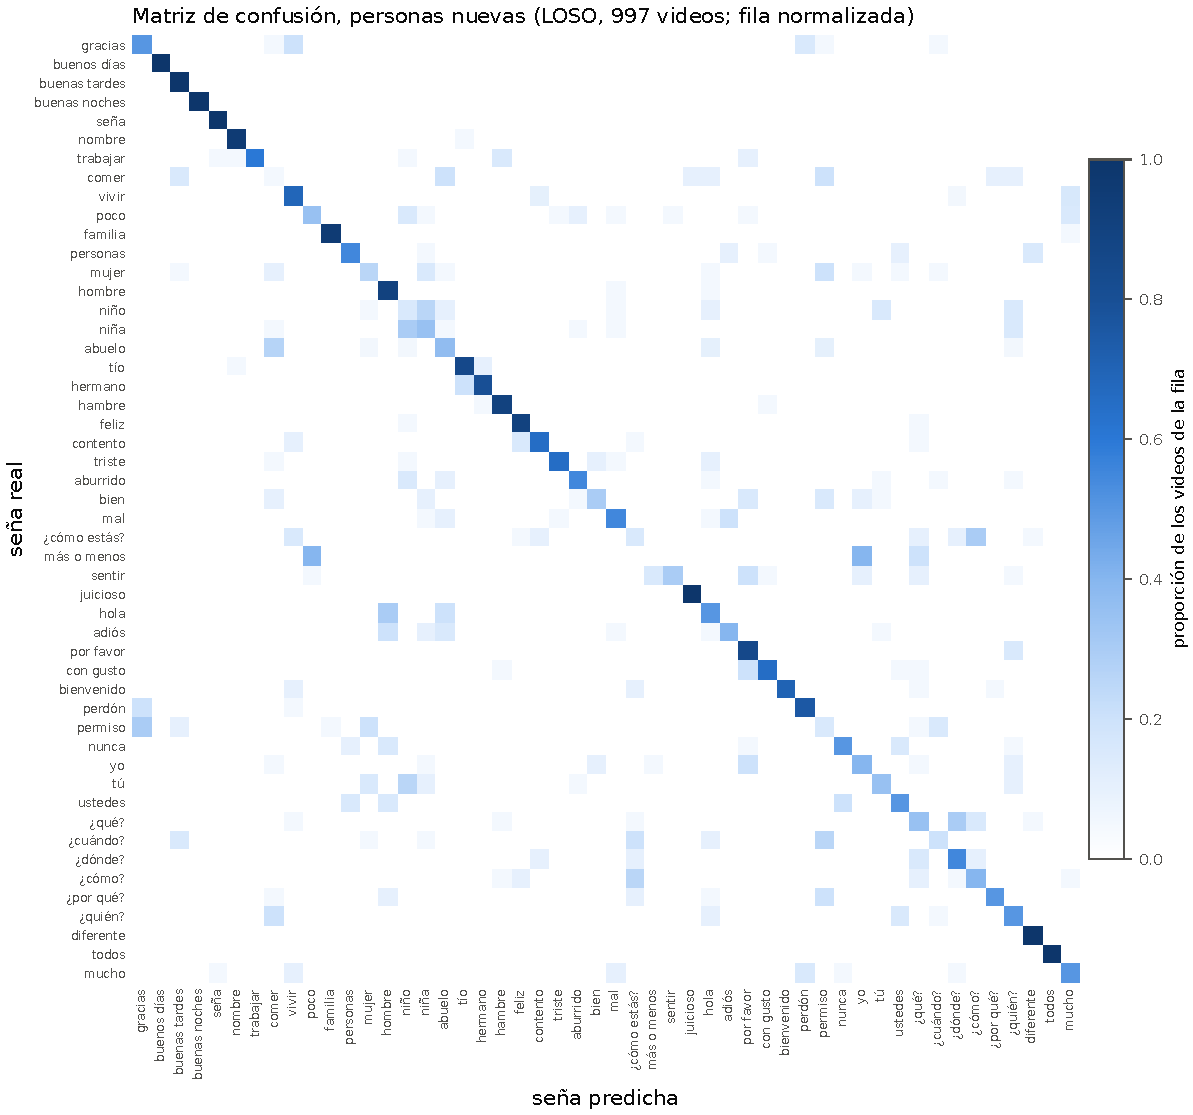
\includegraphics[width=\linewidth,height=6.9cm,keepaspectratio]{res_matriz_confusion_50.pdf}
\fuente{figuras/res\_metricas.json → matriz\_confusion\_997; guion guiones/figuras\_resultados.py (fig\_matriz).}
\end{frame}

% =====================================================================
\begin{frame}{A7. La misma seña dura distinto según la persona que la haga}\label{fr:porsenante}
\centering
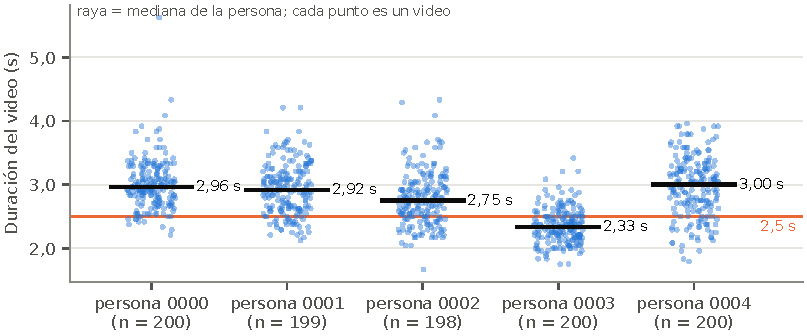
\includegraphics[width=0.85\linewidth,height=4.9cm,keepaspectratio]{fig_duracion_por_senante.pdf}

\small
Medianas: 2,96 / 2,92 / 2,75 / \textbf{2,33} / 3,00 s (personas 0000 a 0004). Es descriptivo: no se analizó su efecto en el LOSO ni se le atribuye causa.
\fuente{guiones/figuras\_datos.py (fig\_duracion\_por\_senante) sobre bitacora\_integridad.json.}
\end{frame}

% =====================================================================
\begin{frame}{A8. Otros hallazgos del EDA: por qué se extrajeron de nuevo los puntos}\label{fr:eda2}
\small
\begin{itemize}\setlength\itemsep{5pt}
  \item En 749 de 1.000 videos, el video tiene más cuadros que filas los archivos de puntos publicados (máx. 51 de diferencia, mediana 5); causa desconocida.
  \item Los puntos del rostro publicados vienen de otra cámara (50 fps) y no se alinean cuadro a cuadro con el cuerpo.
  \item Por eso se extrajeron los puntos de nuevo con MediaPipe HolisticLandmarker sobre los 1.000 videos: 67.328 cuadros, 0 fallidos. Mano izq. detectada en el 93,8 \% de los cuadros, der. en el 97,2 \%; ninguna, 0,44 \%.
  \item Comprobado: los cuadros por video que usa el modelo vigente son exactamente los del video (1.000 de 1.000).
  \item Otros 5 pares idénticos existen solo en cámaras que el proyecto no usa (rostro, profundidad): no afectan el conteo de 997.
  \item Pendientes menores: la glosa 0029 figura como «juicioso» en el código y «Jucioso» en el artículo (va a la validación 1.d).
\end{itemize}
\fuente{caracterizacion.md §7, §10, §11.1; N-02, N-09, N-21; comprobación de lengths.npy frente a bitacora\_integridad.json (pieza «datos» de este flujo).}
\end{frame}

% =====================================================================
\begin{frame}{A9. Glosario (1 de 2): datos y modelo}\label{fr:glosario}
\scriptsize
\renewcommand{\arraystretch}{1.12}
\begin{columns}[T]
\begin{column}{0.49\textwidth}
\begin{tabularx}{\linewidth}{@{}>{\leavevmode\color{azul}\bfseries\raggedright}p{2.1cm} >{\raggedright\arraybackslash\leavevmode}X@{}}
Seña aislada & una seña sola, con inicio y fin, no una frase continua. \\
Glosa & nombre de la seña en español (p. ej. HOLA). \\
Persona (señante) & quien hace las señas en un video; el corpus tiene 5 (0000 a 0004). \\
Cuadro & una imagen del video (24 por segundo, 24 fps, en el corpus). \\
Muestra & un video completo = una seña = una matriz 30 $\times$ 252. \\
Punto clave & \emph{keypoint} o \emph{landmark}: posición (x, y, z) de un lugar del cuerpo. \\
Paso & una de las 30 posiciones en que se reparte la seña. \\
Interpolación lineal & valor intermedio en línea recta entre dos cuadros. \\
Velocidad & cambio de una coordenada entre un paso y el anterior. \\
\end{tabularx}
\end{column}
\begin{column}{0.49\textwidth}
\begin{tabularx}{\linewidth}{@{}>{\leavevmode\color{azul}\bfseries\raggedright}p{2.1cm} >{\raggedright\arraybackslash\leavevmode}X@{}}
Conv1D & capa que recorre la secuencia con ventanas cortas (aquí, 3 pasos) y detecta patrones. \\
LSTM & red recurrente con memoria; bidireccional: lee en los dos sentidos. \\
Atención & pesos por paso que deciden qué momentos importan. \\
Softmax & convierte 50 números en 50 probabilidades que suman 1. \\
GrammarMapper & módulo del prototipo que convierte glosas en una frase en español. \\
Época & una pasada por todo el entrenamiento. \\
Semilla & número que fija el azar del entrenamiento (pesos iniciales, orden de los lotes). \\
Aumentación & copias transformadas de los videos de entrenamiento (espejo, ruido, escala). \\
\end{tabularx}
\end{column}
\end{columns}
\end{frame}

% =====================================================================
\begin{frame}{A10. Glosario (2 de 2): evaluación}\label{fr:glosario2}
\scriptsize
\renewcommand{\arraystretch}{1.12}
\begin{columns}[T]
\begin{column}{0.49\textwidth}
\begin{tabularx}{\linewidth}{@{}>{\leavevmode\color{azul}\bfseries\raggedright}p{2.1cm} >{\raggedright\arraybackslash\leavevmode}X@{}}
Validación & datos que deciden cuándo parar; no ajustan pesos. \\
Prueba & datos evaluados una sola vez al final. \\
LOSO & dejar una persona fuera: se prueba con alguien que el modelo nunca vio. \\
Pliegue & cada una de las 5 particiones del LOSO (una por persona excluida); en la reunión, «universo». \\
Top-1 & exactitud (\emph{accuracy}): la seña correcta es la primera opción. \\
Top-3 & la seña correcta está entre las tres primeras opciones. \\
TP / FN / FP & acierto / seña que se escapa / seña dicha sin que se hiciera. \\
F1 macro & media armónica de precisión y recall, promediada sobre las 50 señas. \\
\end{tabularx}
\end{column}
\begin{column}{0.49\textwidth}
\begin{tabularx}{\linewidth}{@{}>{\leavevmode\color{azul}\bfseries\raggedright}p{2.1cm} >{\raggedright\arraybackslash\leavevmode}X@{}}
Umbral & confianza mínima para decir la seña en voz alta. \\
Utilidad (U) & aciertos dichos menos errores dichos; sirve para elegir el umbral. \\
DE & desviación estándar entre personas (o semillas). \\
IC 95 \% & intervalo de confianza del 95 \%: rango de valores compatibles con los datos. \\
McNemar & prueba estadística que compara dos sistemas sobre los mismos videos. \\
Random Forest, SVM, MLP & clasificadores clásicos: bosque de árboles de decisión, máquina de vectores de soporte y perceptrón multicapa. \\
Línea base & sistema simple con la misma entrada, para saber cuánto aporta la red. \\
\end{tabularx}
\end{column}
\end{columns}
\end{frame}

% =====================================================================
\begin{frame}[fragile]{A11. Cómo correr la prueba de escritorio y el prototipo}\label{fr:comandos}
\small
Desde la raíz del repositorio, con el intérprete del proyecto. Las dos primeras no abren la cámara ni suenan.
\begin{tcolorbox}[colback=grisclaro,colframe=gris!40,boxrule=0.4pt,arc=1pt,left=3pt,right=3pt,top=2pt,bottom=2pt]
{\fontsize{8}{9.6}\selectfont
\begin{verbatim}
# prueba de escritorio de un video (1-2 min); --sin-prototipo omite la 3.a comprobación
python docs/diapositivas_workflow/guiones/prueba_escritorio.py 0030_0000_0000

# la red por dentro con un video del conjunto de prueba («gracias», persona 0003)
python docs/diapositivas_workflow/guiones/pasada_modelo_un_video.py 0000_0003_0002

# prototipo en vivo (desde Terminal.app): ESPACIO abre la ventana de 2,5 s
python src/realtime.py
\end{verbatim}
}
\end{tcolorbox}
\footnotesize Detalle, orden para regenerar todas las figuras y avisos: docs/diapositivas\_workflow/LEEME.md.
\fuente{docs/diapositivas\_workflow/LEEME.md; README.md l. 695 (realtime.py); N-26 (la cámara se abre desde Terminal.app).}
\end{frame}

\end{document}
